\documentclass[a4paper,man,floatsintext,longtable,noextraspace,12pt]{apa6}

\usepackage[english]{babel}
\usepackage[utf8x]{inputenc}
\usepackage{amsmath}
\usepackage{graphicx}
\usepackage[colorinlistoftodos]{todonotes}
\usepackage{hyperref}

\usepackage{booktabs}
\usepackage{longtable}
\usepackage{array}
\usepackage{multirow}
\usepackage{wrapfig}
\usepackage{float}
\usepackage{colortbl}
\usepackage{pdflscape}
\usepackage{tabu}
\usepackage{threeparttable}
\usepackage{threeparttablex}
\usepackage[normalem]{ulem}
\usepackage{makecell}
\usepackage{xcolor}

% bibliography
\newlength{\cslhangindent}
\setlength{\cslhangindent}{1.5em}
\newenvironment{cslreferences}%
  {\setlength{\parindent}{0pt}%
  \everypar{\setlength{\hangindent}{\cslhangindent}}\ignorespaces}%
  {\par}

\renewcommand{\baselinestretch}{1.5}
\setlength\parindent{24pt}


\title{Transparency to hybrid open access invoicing through publisher-provided metadata: A longitudinal article-level study of Elsevier}
\shorttitle{Hybrid OA Elsevier}
% \author{Najko Jahn}
% \affiliation{State and University Library Göttingen, University of Göttingen, Germany}
% \author{Lisa Matthias}
% \affiliation{tba}
% \author{Mikael Laakso}
% \affiliation{tba}
% 

\abstract{The financial flows in scholarly journal publishing have become increasingly complex with the growth of open access (OA), and the lack of data and transparency into these flows has been persistent. Opaqueness has concerned especially hybrid OA, where subscription-based journals also publish OA content if an optional fee is paid. By leveraging Elsevier’s recently introduced article metadata concerning invoiced recipients, this study provides the first longitudinal publisher-level study of uptake and invoicing of hybrid OA articles. The results show that the share of OA articles in Elseviers hybrid journals has grown slowly, from 2.6\% of all articles on average in 2015 to 3.7\% in 2019. About a third of hybrid OA articles are invoiced directly through an agreement with research funders or other type of organisational sponsor (e.g. national library consortia), with the majority invoiced to authors. 83\% of agreement-invoiced hybrid OA articles are to European organisations, suggesting a strong international skewness. The study discovered a large discrepancy in choice of publication license between author-invoiced articles (dominantly CC BY-NC-ND) and agreement-invoiced articles (dominantly CC BY). The results demonstrate the value of publisher-provided metadata covering invoiced recipients of articles, which would be even more useful through wider adoption among publishers.}

\begin{document}
\maketitle

\hypertarget{introduction}{%
\section{Introduction}\label{introduction}}

The rise of open access (OA) to journal articles has added complexity to
scholarly publishing, particularly concerning transparency of economic
dimensions. Financial transparency in journal publishing has long been
lacking since Big Deal subscription contracts between academic
institutions and large academic publishers usually include
confidentiality clauses that prohibit publicly sharing information about
the scope and pricing of such agreements (Bergstrom et al., 2014;
Frazier, 2001; Larivière et al., 2015). Further, the distributed process
of paying for accessing and publishing scholarly articles, which can
involve several actors at the same time, including authors, research
organizations, libraries, and research funders, adds to the opacity of
the financial flows of scholarly publishing (Lawson et al., 2016).

The problem with this lack of transparency becomes more apparent in the
case of hybrid OA. In this OA business model, individual articles can be
made openly available for a fee, also known as article-processing charge
(APC), while the journal as a whole remains subscription access. Hence,
hybrid OA was originally introduced as a low-risk transitional model
that allows journals to gradually convert to full OA and reduce
subscription costs as the OA uptake increases (Prosser, 2003). Many
large subscription publishers have since incorporated this OA model, and
while the uptake among authors increased only slowly during the first
decade (Björk, 2012), it has gradually gained popularity in recent
years. This development was driven by the implementation of OA policies
by research institutions and funders, the allocation of OA funds, and
formal agreements between publishers and institutions that allow
affiliated authors to publish OA free-of-charge (Laakso \& Björk, 2016).
However, there have been concerns that the hybrid model allows for
double-dipping---receiving two payments for one article, the APC and
subscription fees (Prosser, 2015; Shieber, 2009). While publishers
assure they combine subscription fees and APCs to adjust pricing
(Mittermaier, 2015), without transparency around the uptake of hybrid OA
and revenue streams, such claims are impossible to evaluate.

With the recent introduction of transformative agreements, an evolving
term for contracts that shift library spendings for subscriptions to OA
(Borrego et al., 2020; Hinchliffe, 2019), the demand for
publisher-provided data has even increased. If publishers would enable
transparency about the OA uptake in hybrid journals and APC invoicing,
academic libraries could improve their assessments and adjustments of
contracts with publishers (Antelman, 2017; Schimmer et al., 2015).
Likewise, research organizations and funders could improve compliance
monitoring with OA mandates, while ensuring that the different actors
were not charged multiple times (Larivière \& Sugimoto, 2018). However,
as formal bibliometrics and financial studies have noted, the lack of
publicly available and standardized data about hybrid OA publishing is
considerable (Laakso \& Björk, 2016; Lawson, 2015; Pinfield et al.,
2016)

This current study investigates the extent to which publisher-provided
data can be utilized to research hybrid OA. The study takes Elsevier,
the largest scholarly journal publisher in terms of article volume
(Larivière et al., 2015), as the starting point for an empirical
analysis of hybrid OA uptake and invoicing. Our approach is based on
openly available data sources and brings together scholarly metadata
from Crossref, a DOI registration agency for scholarly works, and
machine-readable APC invoicing data from Elsevier OA full-texts. The
so-compiled data enable us to analyze the development of Elsevier's
hybrid journal portfolio from 2015-19, and to compare it with that of
Elsevier's full and delayed OA program. Further, we investigate whether
hybrid publishing fees were waived or charged. In particular, we
identify academic consortia and research funders that were directly
invoiced by Elsevier, and compare their hybrid OA rates by license and
subject. As such, our findings have implications for research and OA
policy and highlight the potential of publisher-provided data for
large-scale, instantaneous analysis of hybrid OA uptake and invoicing.

\hypertarget{background}{%
\section{Background}\label{background}}

The ability to identify and discover hybrid OA articles plays a
fundamental role in monitoring hybrid OA, yet time and again, previous
studies have underscored the difficulties involved in this
(cf.~(Akbaritabar \& Stahlschmidt, 2019; Björk, 2012; Emery, 2013;
Laakso \& Björk, 2016; Leeuwen et al., 2018). Insights into the volume
of hybrid OA and the various levels and sources of APC funding could
create a better understanding of the costs involved in scholarly
publishing and, thus, strengthen institutions' bargaining power in
negotiations with publishers, and promote greater equity in scholarly
publishing. In the following section, we examine how previous research
has tackled the challenge of identifying hybrid OA content and what
these studies taught us about the uptake and funding sources of hybrid
OA.

\hypertarget{prevalence-uptake-studies}{%
\subsection{Prevalence / uptake
studies}\label{prevalence-uptake-studies}}

Since there is no standardized way to measure the uptake of hybrid OA,
estimates can vary greatly depending on how uptake is
operationalized--for example, through the number of hybrid journals with
at least one OA article, the average number of OA articles per hybrid
journal, or the share of OA articles compared to subscription articles.

In the first article-level study on hybrid OA, Laakso \& Björk (2016)
reported that between 2007 and 2013, the five largest
publishers--Elsevier, Sage, Springer, Taylor \& Francis, and
Wiley--recorded growing numbers of hybrid journals that coincided with a
twenty-fold increase in hybrid OA articles (from 666 to 13,994). As a
result, hybrid journals with at least one OA article more than doubled
in number (1,082 in 2009, 2,714 in 2013) but fell by 31\% relative to
the number of hybrid journals in total. Although Laakso and Björk's
(2016) presented a comprehensive overview tracking the growth of hybrid
OA over time and across multiple publishers, their exploratory approach
is unsuitable for repeated use as it required a considerable amount of
manual data collection and cleaning. Minimizing such manual tasks,
Nelson \& Eggett (2017) narrowed their focus to one publisher--the
American Chemical Society (ACS)--and requested a list of all hybrid OA
articles published from 2006-2011 directly from the ACS. To assess the
hybrid OA uptake, the authors aggregated and compared the number of OA
(n=814) and subscription articles (n=27,621), finding that over the five
years, 2.9\% of ACS articles were published as hybrid OA.

Contrary to the previous two studies, Kirkman (2018) took a research
funder as a starting point, reporting a 26\% share of hybrid OA for
articles funded by the Australian National Health and Medical Research
Council from 2012-2014 (816 of 3,190). Kirkman collected research
articles using the Funding Agency and Funding Text search fields on Web
of Science, and classified articles as OA when they were freely
available on the publisher website, and further distinguished hybrid OA
articles based on journal-level information from the publisher website,
such as hybrid OA journal and APC lists. Another approach is presented
by Pölönen et al. (2020), who used current research information system
(CRIS) data---institutional publication data---to study the extent of OA
among Finnish research publications from 2016-2017 (n=34,507 research
articles). As part of the analysis, the authors identified hybrid OA
articles through a dedicated OA status metadata field that has been
mandatory to report in Finland since 2016 and found a 7\% share of
hybrid OA. However, the drawbacks of Kirkman's (2018) and Pölönen et
al.'s (2020) approaches are that such data sources might not be openly
available or, regarding CRIS data, might not be available at all since
not all countries maintain comprehensive institutional publication data.

Other studies assessed the share of (hybrid) OA for the entire corpus of
scholarly research articles. For instance, using research articles with
an assigned DOI and indexed in the Web of Science Core Collection
(n=2,610,305) as a benchmark, Martín-Martín et al. (2018) assessed how
many research articles from 2009 and 2014 are freely available through
Google Scholar. After identifying OA articles through licensing
information from Crossref, the authors estimated the share of hybrid OA
at around 0.5\% in 2009 and 1.5\% in 2014. In a similar vein, Piwowar et
al. (2018) drew on Crossref to identify content licenses. The authors
followed a data-driven approach based on Unpaywall data, which is openly
available and contained 66 million Crossref DOIs at the time, to
determine how much of the scholarly literature is OA. Based on a random
sample of 100,000 Crossref DOIs, the authors found 3.6\% of hybrid OA,
while pointing towards a growing trend in recent years that recorded a
hybrid OA share of 9.4\% of all articles published in 2015.

Since its launch, Unpaywall has become widely used as an OA evidence
source in bibliometric research and rankings(Huang et al., 2020;
Robinson-Garcia et al., 2020). However, results cannot easily be
compared with each other over time because of Unpaywall's ongoing
changes due to non-standardized data to discover hybrid OA. These
changes mainly reflect the growing albeit incomprehensive license
information in Crossref metadata. To overcome these shortcomings, the
developers extended previous web-scraping approaches to better
distinguish between immediate and delayed OA based on licenses at the
date of observation Piwowar et al. (2019). Relatedly, in October 2020,
Elsevier's license for delayed OA content was added to Unpaywall's list
of license patterns (Unpaywall, n.d.-c). At the journal-level, a more
fine-grained identification of full OA journals using OA article
information was developed to better distinguish them from subscription
journals including hybrid journals (Unpaywall, n.d.-b). With its servie
unsub, Unpaywall recently launched a paid service, where libraries can
compare hybrid OA uptake rates with internal financial and usage data to
assess the value of journal subscriptions (Chawla, 2020).

\hypertarget{financial-studies}{%
\subsection{Financial studies}\label{financial-studies}}

Some countries like Sweden and the United Kingdom (UK) have negotiated
national publishing agreements that allow authors to publish hybrid OA
at a discounted fee or for free. These agreements can serve as the basis
for studies on the uptake of hybrid OA or cost-benefit analyses
(cf.~Olsson (2018); Lawson (2017)) but are often limited in scope as
they tend to focus on a single country and rely on data that seldom is
publicly available. Hence, while being valuable for specific use-cases,
such studies can neither provide a comprehensive understanding of how
the scholarly publishing system functions beyond national boundaries nor
facilitate collective sharing of financial information about hybrid OA.

Pinfield et al.'s (2016) analysis of APC payment records provided by 23
UK higher education institutions revealed a sharp increase in central
payments from 2007-2013, which was largely attributed to the
introduction of block grants by Research Councils UK (RCUK) and
non-compliance sanctions by the Wellcome Trust. Moreover, the study
showed that OA fees were paid almost exclusively through RCUK and
Wellcome block grants (92\%), and only a small number of APCs were paid
through internal funding (7\%). In contrast, a recent Springer Nature
survey found that authors draw on a range of funding sources to cover OA
fees, such as dedicated institutional OA funds, block grants, OA
agreements, or research grants (Monaghan et al., 2020). Most hybrid OA
authors were supported through dedicated institutional OA funds (43\%,
excluding block grants) and OA agreements with Springer Nature (34\%).
The differences between these two studies may be due to changes in
policy and funding arrangements---in particular, the introduction of OA
agreements---since Pinfield et al. (2016), or due to Monaghan et al.'s
(2020) more regionally diverse sample, indicating regional differences
in APC funding.

Regional and policy differences in APC payments also came to light in a
study by Jahn \& Tullney (2016) that analyzed APC records from 30 German
higher education and research institutions crowd-sourced by the Open APC
initiative, the Austrian Science Fund (FWF), Jisc, and the Wellcome
Trust. In particular, the study revealed large differences in the amount
of hybrid OA funded from 2014-2015. Whilst hybrid OA accounted for less
than 1\% of APCs paid by German institutions (23 of 3,846), the three
non-German research funders recorded a hybrid share of75\% (11,533 of
15,779). According to Jahn \& Tullney (2016), this could point towards
differences in science policy, such as hybrid OA being supported by the
three non-German research funders but not by Germany's largest national
funder (DFG). Another possibility is that German hybrid OA fees were
paid from budgets not reported to the Open APC initiative, from where
the authors acquired the German APC data. Among these unreported funds
are research grants and research unit budgets, which author surveys
identified as funding sources for hybrid OA fees (Graaf, 2017; Monaghan
et al., 2020). As such, Jahn and Tullney's (2016) findings could reflect
the complexities and potential limitations of institutional OA spending
data that Pinfield et al.~(2016) and Monaghan et al.~(2020) attributed
to incomplete or missing records.

As this brief review has shown, the most comprehensive studies approach
hybrid OA funding from an institutional perspective that focuses on
research institutions or funders and draws on internal records or
crowd-sourced data like from the Open APC initiative. The advantages of
Open APC data are that they reflect the actual APCs paid rather than
list prices; they are not limited to certain publishers or journals;
they are provided in a standardized format regardless of the publisher.
On the other hand, the drawbacks include the limited number of
participating institutions that are almost exclusively based in Europe
and the dependency on participating organizations for data integrity
(Pieper \& Broschinski, 2018). Moreover, since Open APC data does not
include waivers or free APCs, it cannot present a complete picture of
all publishing activities and expenses. This, however, would pose less
of an issue when analyzing just hybrid OA.

\hypertarget{the-role-of-publisher-provided-data}{%
\subsection{The role of publisher-provided
data}\label{the-role-of-publisher-provided-data}}

Uptake and financial studies have OA policy implications for hybrid OA.
Most prominently, the cOAlition S, an international network of research
funders, released its widely discussed Plan S. In September 2018, the
cOAlition S announced that from 2021 onwards, signatories would no
longer fund articles in hybrid OA journals. This principle includes
so-called ``mirror'' and sister journals--hybrid journals with fully OA
counterparts or split into their fully OA and subscription parts---that
have launched since Plan S was announced but makes an exception for
hybrid journals with transformative agreements (Frantsvåg \& Strømme,
2019). The Plan S refers to the Efficiency and Standards for Article
Charges (ESAC) guidelines (Geschuhn \& Stone, 2017) as critical
component of transformative agreements, emphasizing the need for
publisher-provided metadata to address the lack of transparency
surrounding hybrid OA. However, studies confirm that publisher with such
agreements lack essential data about hybrid OA uptake and invoicing, or
are not able or willing to provide such information publicly and
instantaneously (Marques et al., 2019; Monaghan et al., 2020), which, in
turn, not just limit the monitoring of hybrid OA, but also research
studies on its size and financial implications.

Here, we focus on Elsevier. The publisher provides article-level
metadata to Crossref, including license information, which can be used
to identify OA articles, and links to HTML and XML full-text versions
for text and data mining purposes. Surprisingly, besides the full-text
article, the XML files also contain invoicing information and the
article's OA status. Table \ref{tab:els_xml} summarizes the key metadata
elements, which comprise the type of entity to which the APC was
invoiced (\texttt{openaccessSponsorType}) and the name of that entity if
available (\texttt{openaccessSponsorName}). Moreover, the article-level
metadata indicates if OA was provided through Elsevier's Open Archive
program (\texttt{openArchiveArticle}), which enables free access to
participating subscription journals after an embargo period (i.e.,
delayed OA; Elsevier (n.d.-b)). As we have been unable to identify
similar efforts by other large publishers (e.g., Springer Nature), this
increased transparency through openly available bibliometric and
financial data at the article level seems unique to Elsevier.

\begin{table}[H]
\caption{\label{tab:els_xml} Overview of hybrid open access (OA) uptake across Elsevier hybrid journals with at least one OA article 2015-2019}
\centering
\begin{tabular}[t]{lp{10cm}}
\toprule
XML Node & Description\\
\midrule
\texttt{openaccessArticle} & Indicates if the article is open
access. \\
\texttt{openaccessSponsorType} & Invoice recipient type.\\
\texttt{openaccessSponsorName} & Entity that received Elsevier's APC
invoice.\\
\texttt{openArchiveArticle} & Indicates if open access was provided through
Elsevier's Open Archive programme.\tabularnewline \\
\bottomrule
\end{tabular}
\end{table}

In this study, we utilize Elsevier's publicly available metadata to
analyze the uptake and invoicing of their hybrid OA publishing option.
In particular, we use this novel methodology to answer the following
questions:

\begin{itemize}
\item
  What was the uptake of Elsevier's hybrid OA publishing option between
  2015 and 2019?
\item
  Through which channels were hybrid APCs invoiced, and who were the
  recipients?
\end{itemize}

\hypertarget{methodology}{%
\section{Methodology}\label{methodology}}

For this study, we collected data relating to Elsevier's hybrid OA
option by drawing on multiple freely available data sources. We
identified Elsevier hybrid journals through Elsevier's APC list and
supplemented our sample with Crossref metadata and text-mined invoicing
data to investigate the financing of immediate OA articles provided
under a Creative Commons license in subscription-based journals. Figure
\ref{fig:workflow} visualizes the automated workflow we used to collect
data from Elsevier and Crossref.

\begin{figure}[H]

{\centering 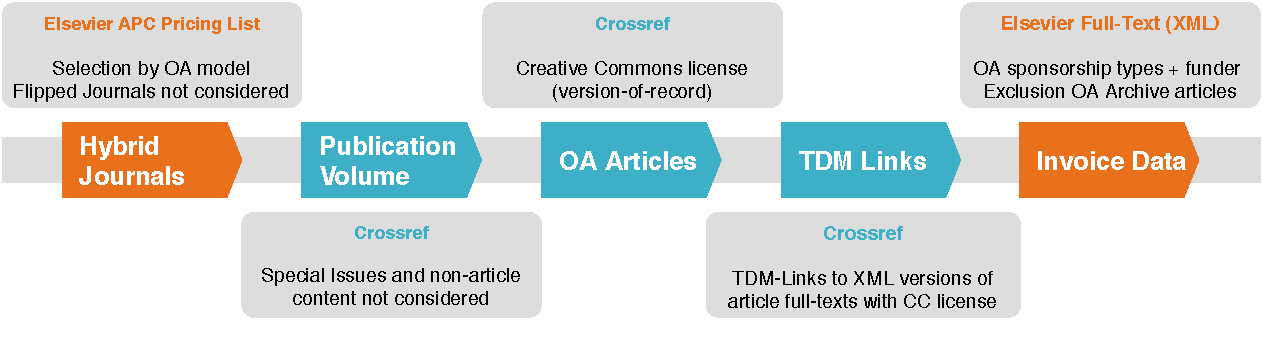
\includegraphics[width=0.95\textwidth]{../figure/els_flow.pdf}

}

\caption{Data Analytics Workflow to obtain article-level OA and invoicing data using freely available data sources provided by Elsevier and Crossref.
}\label{fig:workflow}
\end{figure}

First, we obtained hybrid journals through an Elsevier APC price list
from May 2020 provided as captured by Matthias (2020). We only included
hybrid journals that were published under the hybrid model throughout
the entire period of our analysis. Hence, we excluded journals that
flipped from OA to hybrid and from hybrid to OA. This approach allowed
us to ensure that the article-level differences we observed were not due
changes at the journal-level (i.e., increases or decreases in number).
Overall, we identified 1,970 unique hybrid journals.

Next, we used an openly available Crossref database snapshot (Crossref,
2020), which contains all Crossref records registered until March 2020,
to calculate the journals' combined article volume for the five-year
period from 2015-2019. We only included articles published in regular
issues aside from supplements containing conference contributions like
meeting abstracts, indicated by non-numeric pagination. We excluded
non-scholarly journal content, such as the table of contents and lists
of reviewers, following Unpaywall's paratext recognition approach
(Unpaywall, n.d.-a), which we expanded to include patterns indicating
corrections. Furthermore, we categorized the articles by subject
according to the All Science Journal Classification code (ASJC) and
added citation indicators from the Scopus Source Title list (version
June 2020) based on the journal they were published in.

Crossref metadata also contains license information that indicates if
and under which terms the publisher has made articles openly available
on their website (Hendricks et al., 2020). We identified OA articles
through Creative Commons (CC) licenses and then downloaded the XML
version of all CC-licensed articles published in a hybrid journal. From
the XML files, we determined whether or not the articles were immediate
OA using the XML node \texttt{openArchiveArticle} and measured the
uptake of hybrid OA through three bibliometric indicators (Laakso \&
Björk, 2016; Nelson \& Eggett, 2017)-\/---the number of hybrid journals
with at least one OA article, the number of hybrid OA articles, and the
number of hybrid OA articles relative to the number of closed-accessed
articles in hybrid journals with at least one OA article.

Moreover, we obtained APC invoicing metadata from the XML (see Table 1),
which enabled us to identify the invoice channels and recipients of
hybrid OA APCs. Based on the \texttt{openaccessSponsorType} node in the
XML files, we distinguish between four invoice channels, including
invoices billed to the corresponding author, as part of publishing
agreements with funding bodies (hereinafter ``agreements''; cf.~Elsevier
(n.d.-a)), fee waivers (e.g., in ``cases of genuine need'' or due to
society or university sponsorships, cf.~ref), and other types not
specified by Elsevier. Finally, when hybrid APCs were invoiced as part
of OA agreements, we identified invoice recipients through the
\texttt{openaccessSponsorName} node.

We manually classified invoice recipients based on their institutional
sectors, countries, and primary research areas. Following the OECD's
Frascati Manual (OECD, 2015, p. 91), we coded for four sectors, business
enterprise, government, higher education, and private non-profit. The
government sector consists of federal, state, and municipal governments,
plus non-profit institutions controlled by government units (OECD, 2015,
p. 100). The higher education sector comprises institutions that perform
research and development and provide formal tertiary education services,
such as universities or research institutes (OECD, 2015, p. 101). Legal
or social entities that produce goods and services without generating
profit, such as learned societies or charities, constitute the private
non-profit sector (OECD, 2015, p. 288). Due to the low article volume,
we combined invoice recipients Elsevier listed as ``authors'' and
``third-party sponsor'', and those we had coded as business enterprises
(OECD, 2015, p. 97), into ``Others''. Moreover, we categorized invoice
recipients according to the country or countries representing their
scope of funding and based on the following primary research areas
health sciences, life sciences, physical sciences and mathematics,
social sciences and humanities, unknown, and broad (i.e., multiple
research areas).

It is important to note that we could not find any official
comprehensive documentation of Elsevier's XML schema , at the time of
writing. However, our conceptualization of the variables and
interpretation of the data was informed by a comprehensive review of
Elsevier's websites about OA, including a list of funding agreements and
details about Elsevier's Open Archive program,and Elsevier's article
submission process in the context of dedicated OA agreements (Elsevier,
n.d.-d, n.d.-e, n.d.-c). For validation, we matched the invoicing data
provided by Elsevier to data from the Open APC initiative.

Throughout the mostly automated data gathering and analysis process, we
used tools from the Tidyverse (Wickham et al., 2019) for the R
programming language (R Core Team, 2020). To allow for efficient data
manipulation and retrieval, we imported the Crossref dump to Google
BigQuery, applying the rcrossref (Chamberlain et al., 2020) parsers to
extract relevant metadata fields. We interfaced Google BigQuery with SQL
with the bigrquery client (Wickham \& Bryan, 2020). We used crminer
(Chamberlain, 2020) to obtain the XML files from Elsevier and the xml2
package (Wickham et al., 2020) to parse relevant metadata. To ensure our
results are reproducible, we provided all code for obtaining the data
and performing the analyses with detailed documentation as RMarkdown
notebooks on GitHub
(\url{https://github.com/njahn82/elsevier_hybrid_invoicing}).

\hypertarget{results}{%
\section*{Results}\label{results}}
\addcontentsline{toc}{section}{Results}

This section first presents the results of our analysis of hybrid OA
uptake in Elsevier's journal portfolio with a view to licensing,
disciplinary differences, and citation impact. Then, we present a
descriptive analysis of Elsevier's invoicing data, highlighting
licensing and disciplinary differences for different invoicing channels,
institutional sectors, and individual invoice recipients.

\hypertarget{uptake-of-hybrid-open-access}{%
\subsection*{Uptake of Hybrid Open
Access}\label{uptake-of-hybrid-open-access}}
\addcontentsline{toc}{subsection}{Uptake of Hybrid Open Access}

\hypertarget{overview}{%
\subsubsection*{Overview}\label{overview}}
\addcontentsline{toc}{subsubsection}{Overview}

Between 2015 and 2019, 1,755 of 1,970 (89.1\%) hybrid journals published
at least one OA article. Together these journals published 71,643 OA
articles, which represents 3\% of their total article volume
(n=2,422,087). Table \ref{tab:overview} presents these findings for each
year and the aggregated five-year period, illustrating a moderate growth
in hybrid OA over time. With each year, the number of hybrid journals
with at least one OA article increased, as did the number of immediate
OA articles in these journals, which nearly doubled from 10,672 in 2015
to 19,311 in 2019. However, since the total number of articles published
in these journals also grew over time, the relative share of OA articles
in hybrid journals only increased slightly from 2.6\% to 3.7\%.

\begin{table}[H]

\caption{\label{tab:overview}Overview of hybrid open access (OA) uptake across Elsevier hybrid journals with at least one OA article 2015-2019.}
\centering
\begin{tabular}[t]{lrrrrrr}
\toprule
  & 2015 & 2016 & 2017 & 2018 & 2019 & 2015-19\\
\midrule
\addlinespace[0.3em]
\multicolumn{7}{l}{\textbf{Elsevier Hybrid Journals with ≥ 1 OA article}}\\
\hspace{1em}Total & 1,317.0 & 1,364.0 & 1,401.0 & 1,501.0 & 1,600.0 & 1,755.0\\
\addlinespace[0.3em]
\multicolumn{7}{l}{\textbf{Articles in Elsevier Hybrid Journals with ≥ 1 OA Article}}\\
\hspace{1em}Total & 406,701.0 & 422,423.0 & 436,418.0 & 468,952.0 & 518,062.0 & 2,422,087.0\\
\hspace{1em}Avg. & 308.8 & 309.7 & 311.5 & 312.4 & 323.8 & 1,380.1\\
\hspace{1em}SD & 401.1 & 419.6 & 427.5 & 445.6 & 479.9 & 1,937.5\\
\addlinespace[0.3em]
\multicolumn{7}{l}{\textbf{OA Articles in Elsevier Hybrid Journals with ≥ 1 OA Article}}\\
\hspace{1em}Total & 10,672.0 & 12,729.0 & 13,361.0 & 15,570.0 & 19,311.0 & 71,643.0\\
\hspace{1em}Avg. & 8.1 & 9.3 & 9.5 & 10.4 & 12.1 & 40.8\\
\hspace{1em}SD & 12.9 & 19.7 & 15.6 & 16.2 & 20.1 & 68.9\\
\addlinespace[0.3em]
\multicolumn{7}{l}{\textbf{OA Uptake in Elsevier Hybrid Journals with ≥ 1 OA Article}}\\
\hspace{1em}Total (\%) & 2.6 & 3.0 & 3.1 & 3.3 & 3.7 & 3.0\\
\hspace{1em}Avg. & 3.7 & 4.3 & 4.4 & 4.7 & 5.4 & 3.8\\
\hspace{1em}SD & 4.5 & 5.9 & 5.1 & 4.9 & 5.7 & 4.1\\
\bottomrule
\end{tabular}
\end{table}

Figure \ref{fig:boxuptake} presents the hybrid OA uptake by year,
showing considerable variation among Elsevier's hybrid journals. The
box-and-whiskers plot visualizes the median hybrid OA uptake (horizontal
line inside the box), the range of the majority of journals (the box),
and individual outliers (dots). Notably, the upper quartiles and
whiskers stretch farther over the years, which indicates that the range
of uptake among journals with an above-average proportion of OA articles
increased over the years. Nevertheless, the prevalence of hybrid OA
remained relatively low; in 2019, 95\% of Elsevier hybrid journals
published ≤15.6\% of their articles OA.

\begin{figure}[H]

{\centering 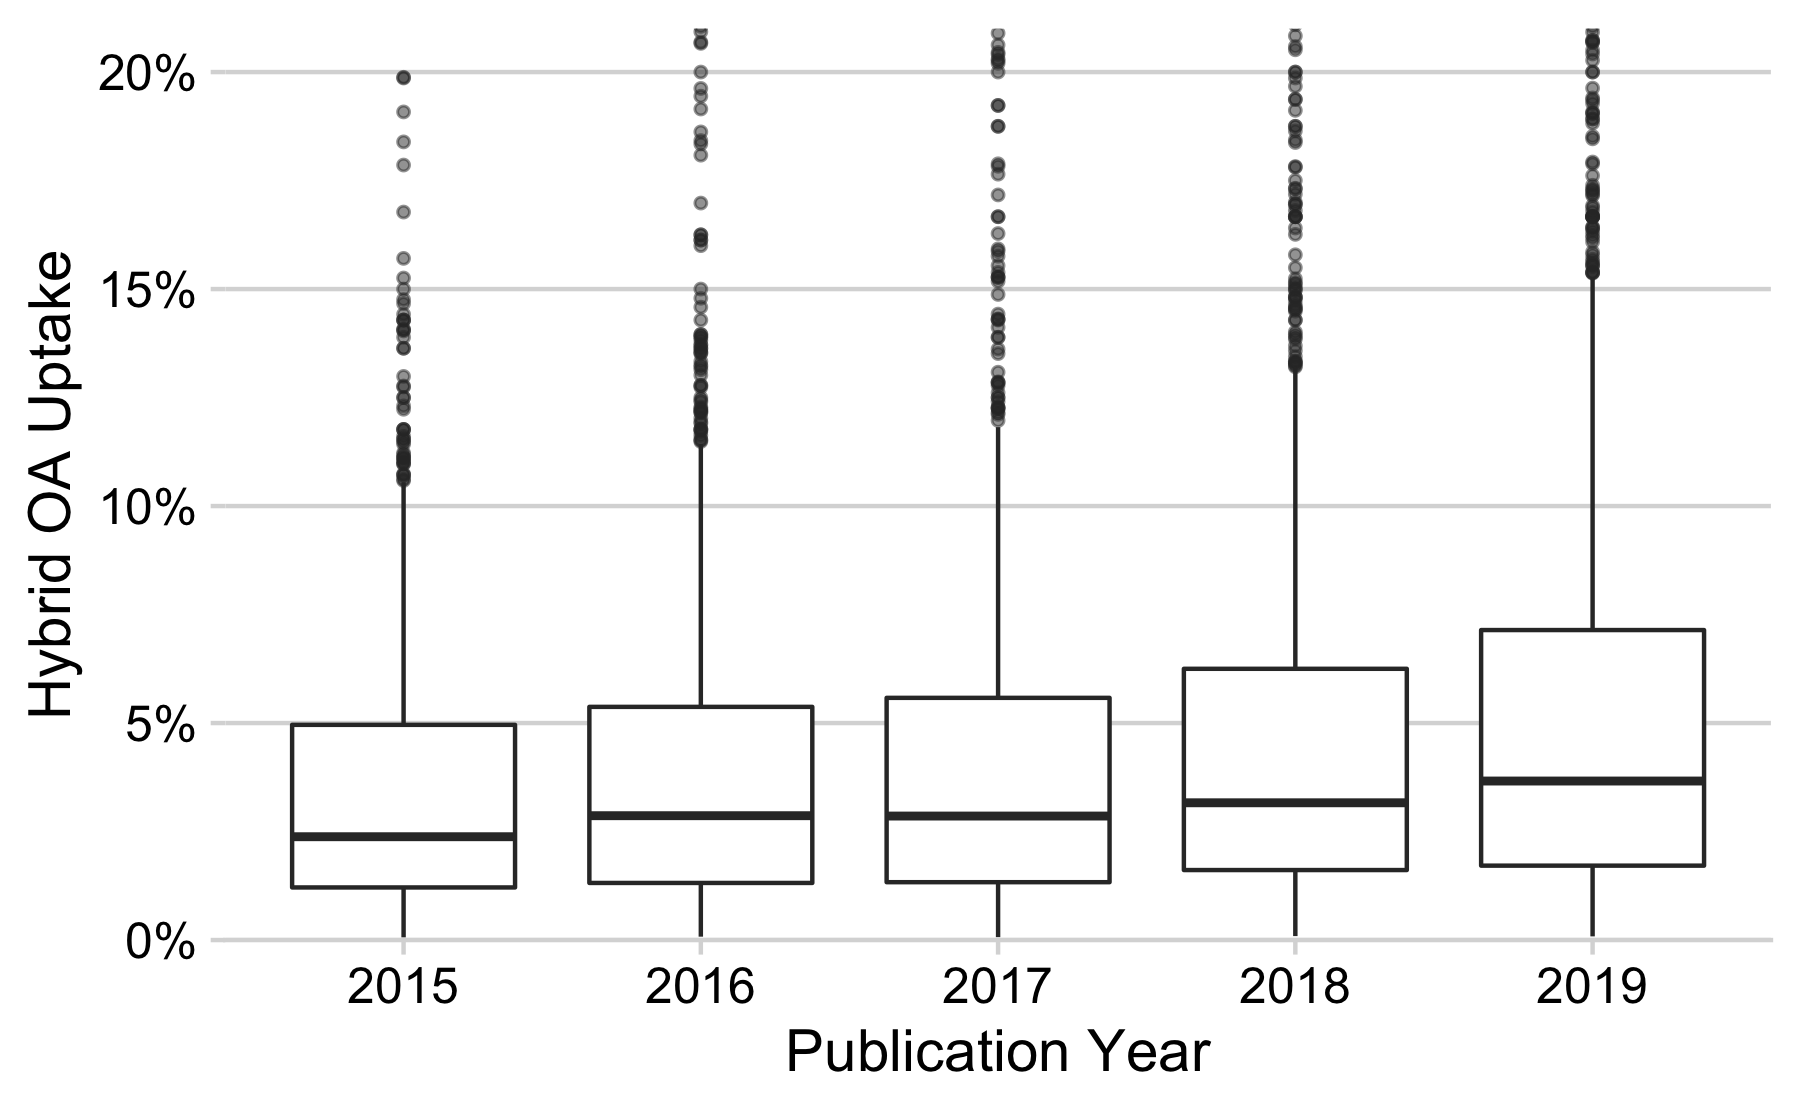
\includegraphics[width=0.7\linewidth,]{manuscript_files/figure-latex/boxuptake-1} 

}

\caption{Open access uptake per Elsevier hybrid journal in percent by year, visualized as box-and-whiskers plot. The Y-axis is limited to an open access share of 20\%.}\label{fig:boxuptake}
\end{figure}

\hypertarget{share-of-the-total-volume-published-in-oa}{%
\subsubsection*{Share of the Total Volume published in
OA}\label{share-of-the-total-volume-published-in-oa}}
\addcontentsline{toc}{subsubsection}{Share of the Total Volume published
in OA}

During the same period, Elsevier published 328,601 OA articles in total
(i.e., in hybrid and full OA journals), representing 12.4\% of the total
article volume (n=2,643,474). Looking at Figure \ref{fig:oa_volume_fig},
it is apparent that the OA article volume of hybrid journals (n=71,643;
21.8\%) lagged behind that of Elsevier's Open Archive program
(n=163,643; 49.8\%) and full OA journals (n=93,315; 28.4\%), which
included 817 articles published in 38 mirror journals.

\begin{figure}[H]

{\centering 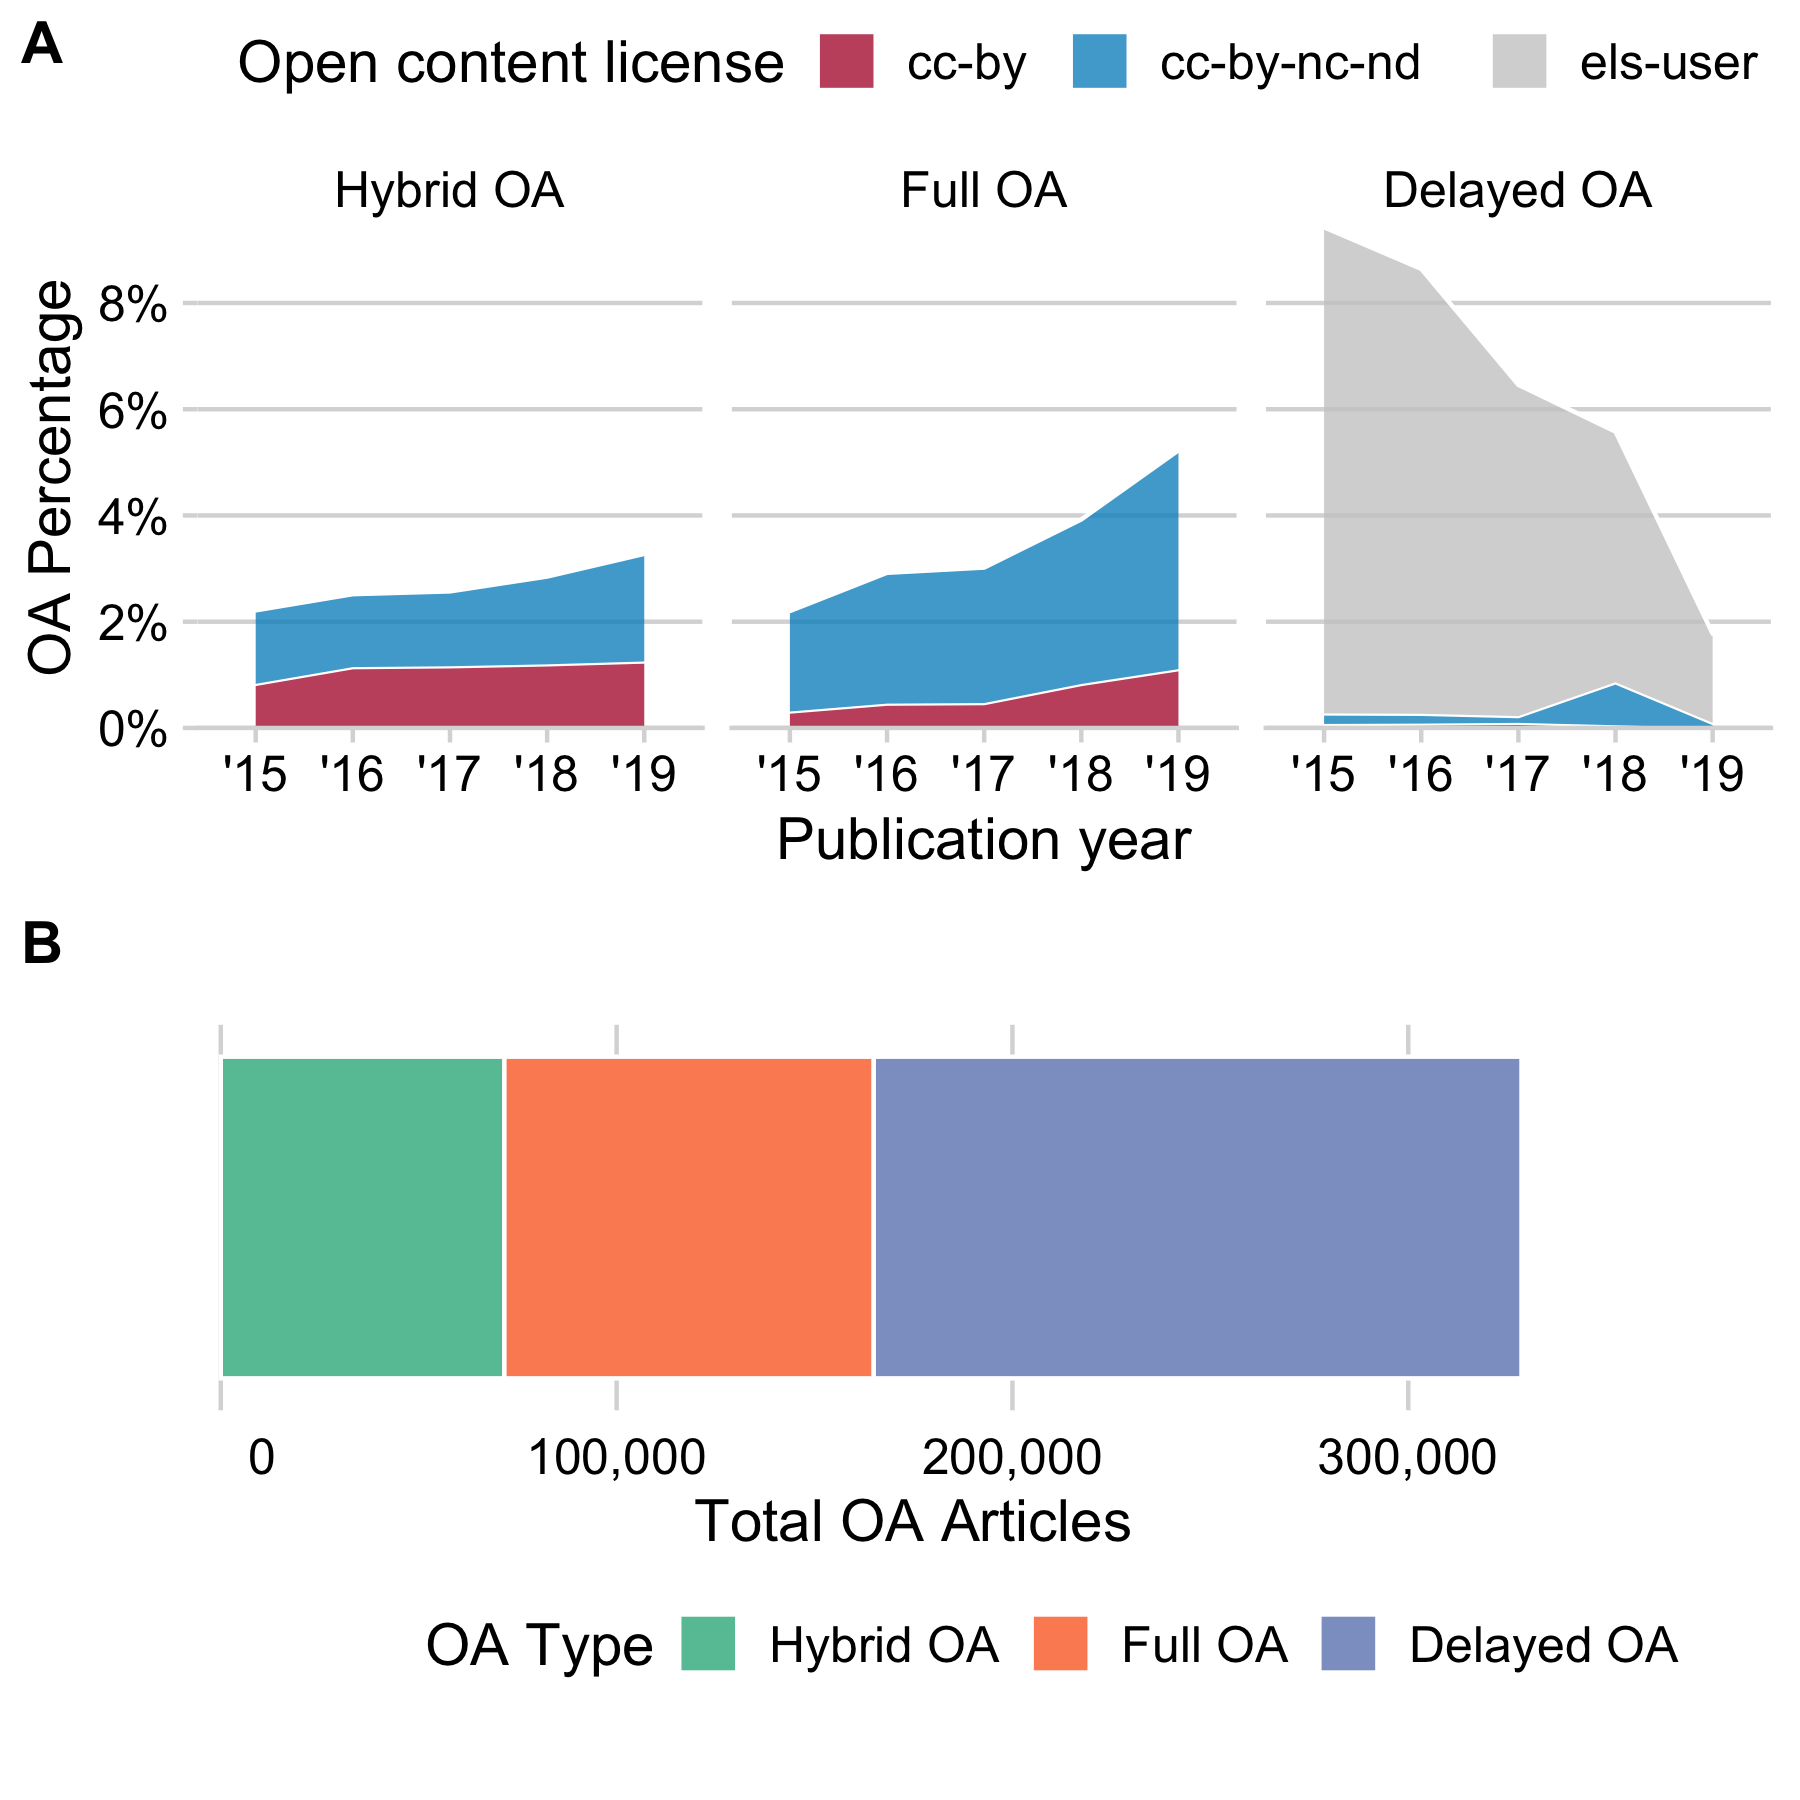
\includegraphics[width=0.7\linewidth,]{/Users/najkojahn/Documents/papers/elsevier_hybrid_invoicing/figure/license_portfolio} 

}

\caption{Open Access (OA) in Elsevier journals in terms of article volume between 2015-2019. Figure A presents the aggregated OA article volume of Elsevier journals from 2015-2019 by OA type. Figure B presents the share of OA articles relative to Elsevier's overall article output by OA type and open content license from 2015-2019.}\label{fig:oa_volume_fig}
\end{figure}

\hypertarget{license-prevalence}{%
\subsubsection*{License Prevalence}\label{license-prevalence}}
\addcontentsline{toc}{subsubsection}{License Prevalence}

As far as we observed, OA articles in Elsevier hybrid journals were
published under two possible CC licenses--CC BY or CC BY-NC-ND. CC BY
allows others to distribute, remix, adapt, and build upon the licensed
work, including for commercial purposes, as long as the original author
is credited. In contrast, CC BY-NC-ND is less permissive as it prohibits
commercial reuse and derivatives. In the five-year period from
2015-2019, the proportion of hybrid OA articles published under a CC
BY-NC-ND license marginally increased and maintained a greater share
than that of CC BY (see Figure \ref{fig:oa_volume_fig}-B).
Interestingly, Figure \ref{fig:oa_volume_fig}-B also reveals that hybrid
journals had the highest number and proportion of openly available
articles licensed under CC BY (n=29,752; 41.5\%) compared to full OA
journals (n=17,293; 18.5\%) and Elsevier's delayed OA program (n=1,568;
1\%) . Most delayed OA articles were provided under an Elsevier user
license (Els-User), which prohibits reuse for commercial purposes.

\hypertarget{subject-area-and-field}{%
\subsubsection*{Subject Area and Field}\label{subject-area-and-field}}
\addcontentsline{toc}{subsubsection}{Subject Area and Field}

Next, we present disciplinary variations in hybrid OA. Table
\ref{tab:subject_area_table} presents the high-level findings by AJSC
subject area. In the five-year period we studied, the physical sciences
(712 hybrid journals, 29,584 OA articles) and health sciences (634
hybrid journals, 25,119 OA articles) were the most prevalent in terms of
hybrid journals with at least one OA article. In terms of article
volume, most OA articles were published in hybrid journals belonging to
the life sciences (538 hybrid journals, 31,383 OA articles), while
social sciences (372 hybrid journals, 11,204 articles) journals
published the lowest number of OA articles. However, it is important to
note that there is a large overlap between the journals' subject areas.
Therefore, Table \ref{tab:subject_area_table} also assigns hybrid
journals and OA articles fractionally to a subject area and compares it
to the full counting, where journals assigned more than one subject in
the AJSC classification were counted once for each field. For the
remaining results, we only present the full counting.

\begin{table}

\caption{\label{tab:subject_area_table}Subject area overview using full and fractional counting. Table reports the number of Elsevier hybrid journals with at least one open access (OA) article, and OA articles published from 2015-2019. One multidisciplinary with 61 OA articles and 11 journals with 37 OA articles that  could not be matched to the Scopus Source Title list used to obtain ASJC codes are not included.}
\centering
\begin{tabular}[t]{lrrrr}
\toprule
\multicolumn{1}{c}{ } & \multicolumn{2}{c}{Full counting} & \multicolumn{2}{c}{Fractional counting} \\
\cmidrule(l{3pt}r{3pt}){2-3} \cmidrule(l{3pt}r{3pt}){4-5}
Subject area & Journals & OA articles & Journals & OA articles\\
\midrule
Health sciences & 634 & 25,119 & 506.6 & 18,415\\
Life sciences & 538 & 31,383 & 368.5 & 21,753\\
Physical sciences & 712 & 29,584 & 584.4 & 23,915\\
Social sciences & 372 & 11,204 & 283.5 & 7,462\\
\bottomrule
\end{tabular}
\end{table}

Figure \ref{fig:oa_sub_uptake} presents the journals' five-year OA
uptake grouped by subject area and field and in comparison to the
overall median (Mdn= 2.5; excluding one journal coded as
multidisciplinary). The box plot reveals some variation between the
subject areas. Notably, with the exception of environmental science and
earth and planetary sciences, journals from the physical sciences show a
lower median proportion of hybrid OA articles, whereas most life
sciences and social sciences journals ranked above average. Figure X
also shows large variations among the 26 subject fields, with the
highest OA rates in immunology and microbiology (Mdn=5.1), environmental
science (Mdn=4.8), and neuroscience (Mdn=4.3), whilst chemistry
(Mdn=1.4), materials science (Mdn=1.4), and dentistry (Mdn=0.6) recorded
the lowest OA rate.

\begin{figure}[H]

{\centering 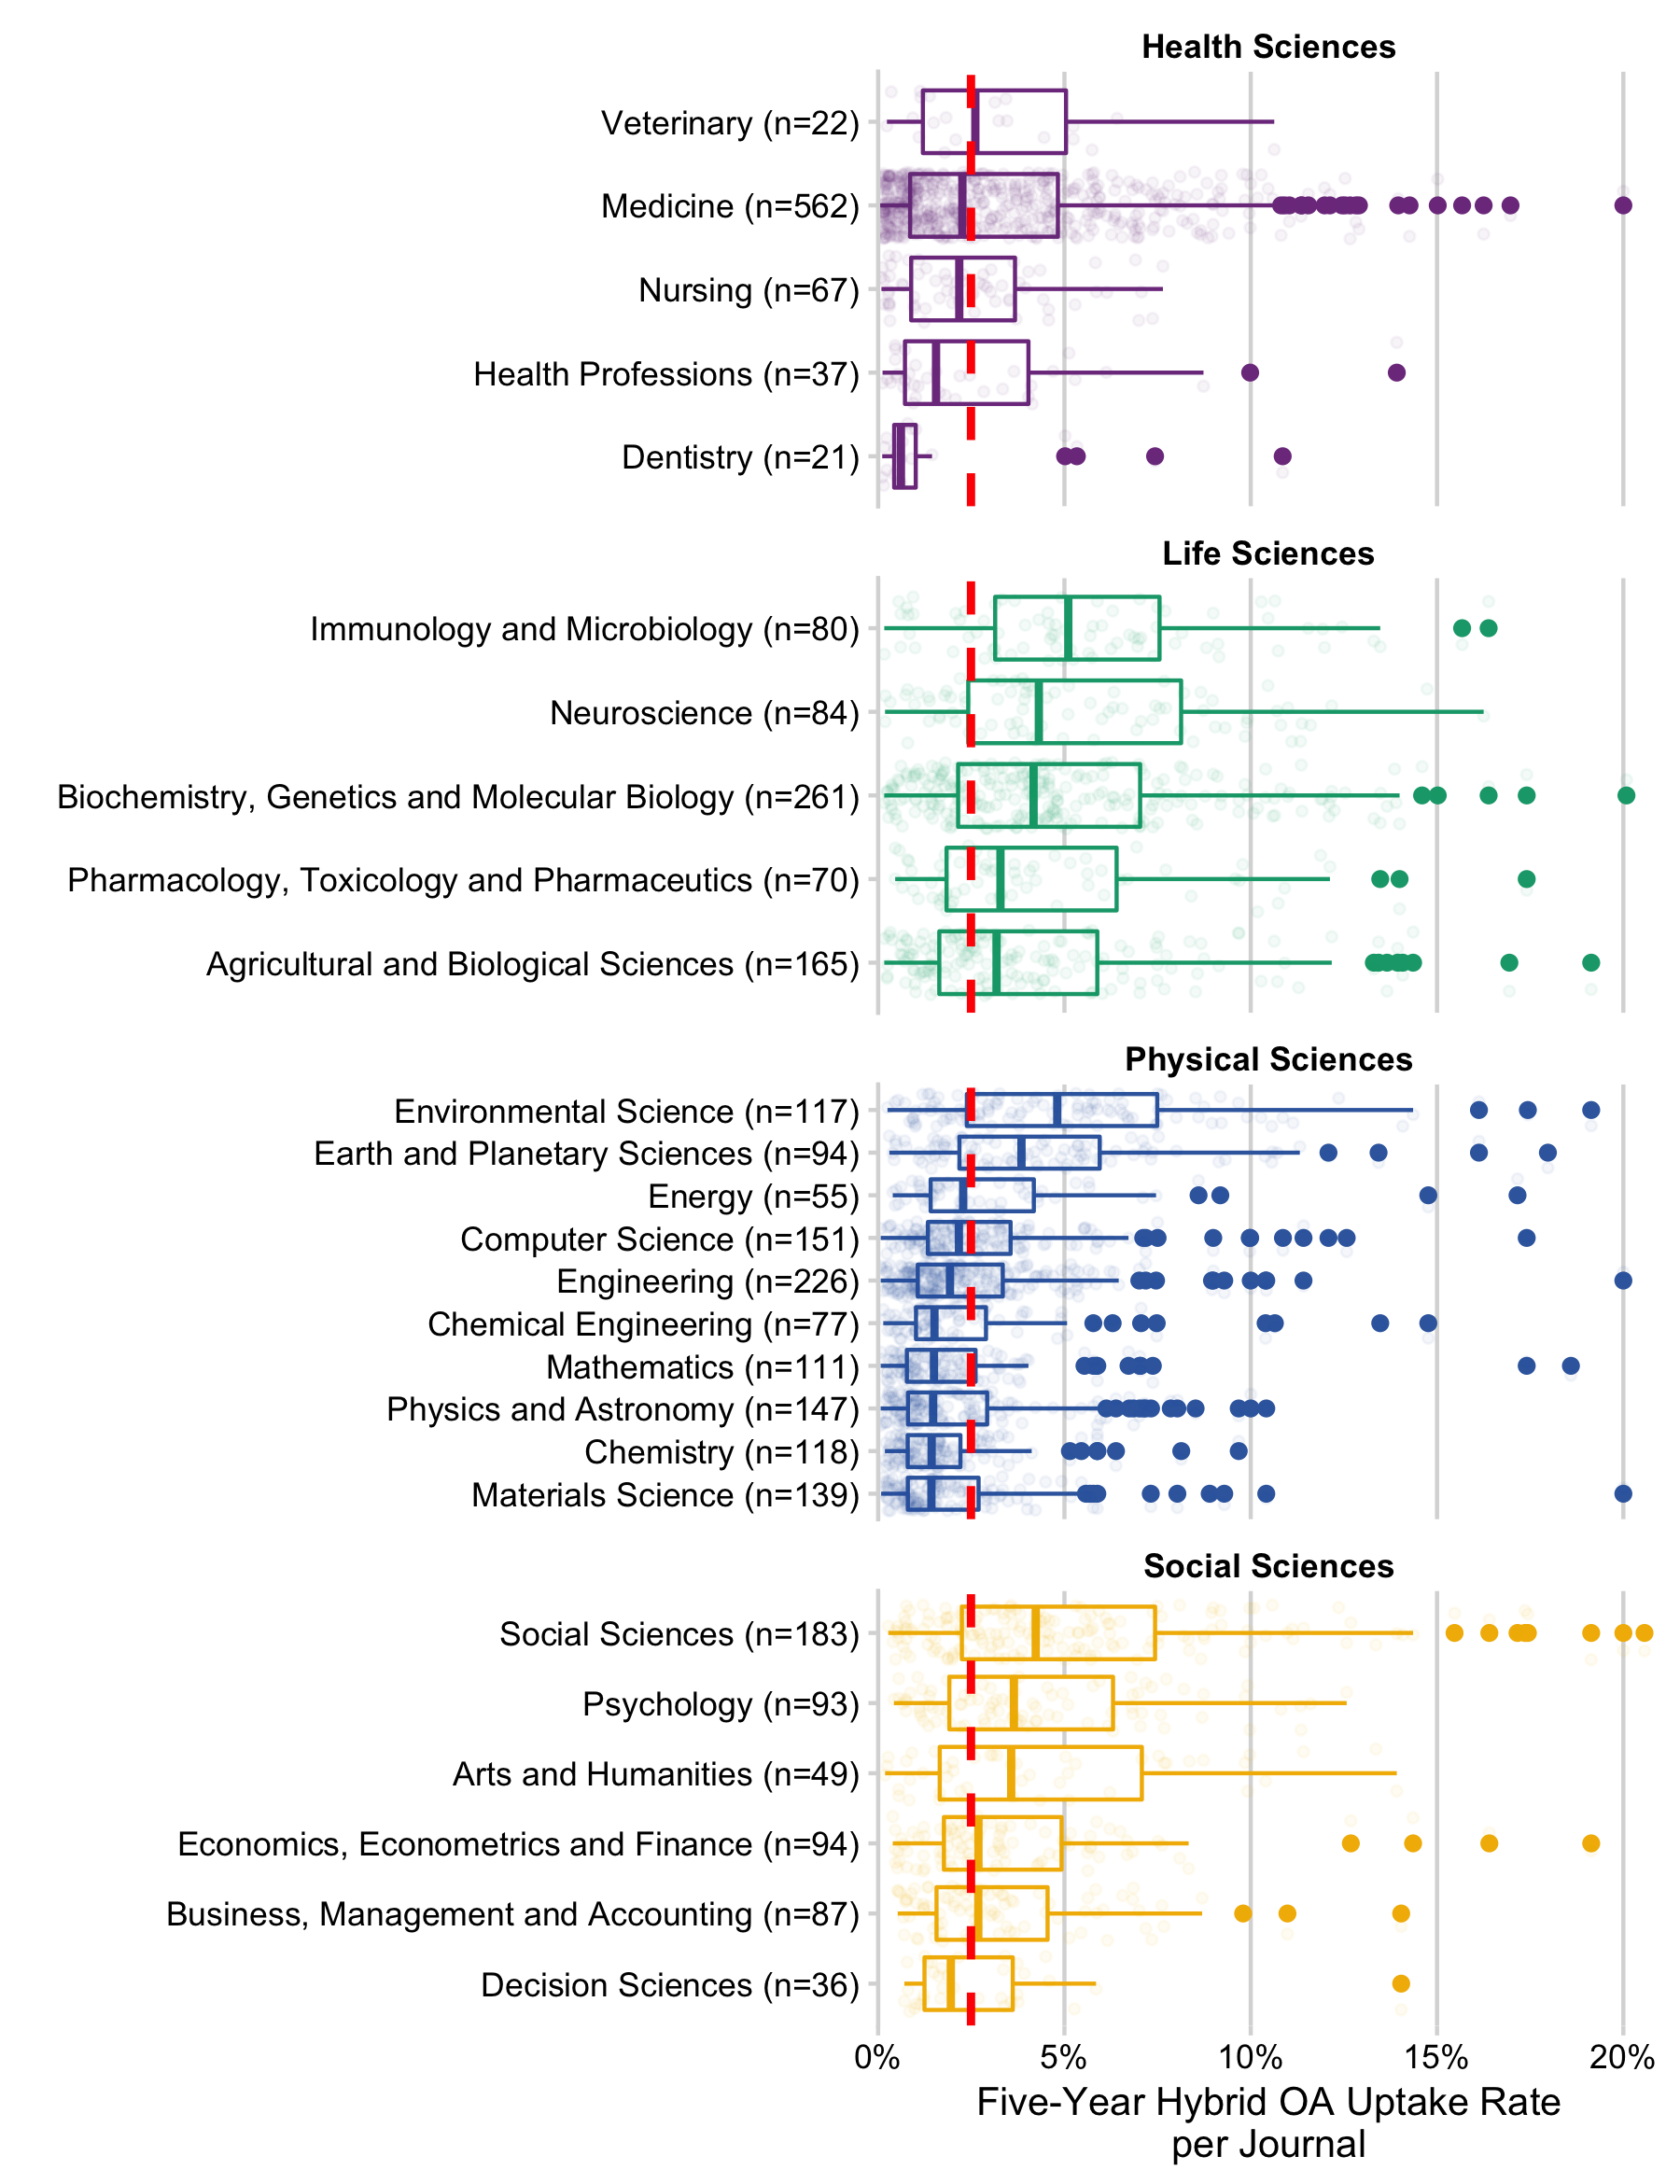
\includegraphics[width=0.9\linewidth,]{manuscript_files/figure-latex/oa_sub_uptake-1} 

}

\caption{Open access (OA) uptake in Elsevier hybrid journals in percent grouped by subject area and field between 2015-19. Visualized as a box-and-whiskers plot limited to an OA share of 20\%; the red line represents the overall median (2.5), jittered dots represent individual journals. Subject fields are ordered based on the median OA uptake.}\label{fig:oa_sub_uptake}
\end{figure}

\hypertarget{citation-impact}{%
\subsubsection*{Citation Impact}\label{citation-impact}}
\addcontentsline{toc}{subsubsection}{Citation Impact}

Furthermore, we were interested in the relationship between the
journals' field-specific impact and their OA uptake. Spearman's rho
correlation coefficient was used to assess the relationship between the
2019 Source Normalized Impact per Paper (SNIP) value calculated by
Scopus and the journals' OA uptake that year. Considering only journals
with at least one OA article, we found a weak but positive correlation
between journal impact and OA uptake (\(r_s\)=0.1679, \(p<0.001\)),
suggesting that the relationship is not very strong, based on our data
(see Figure \ref{fig:sniptest}).

\begin{figure}[H]

{\centering 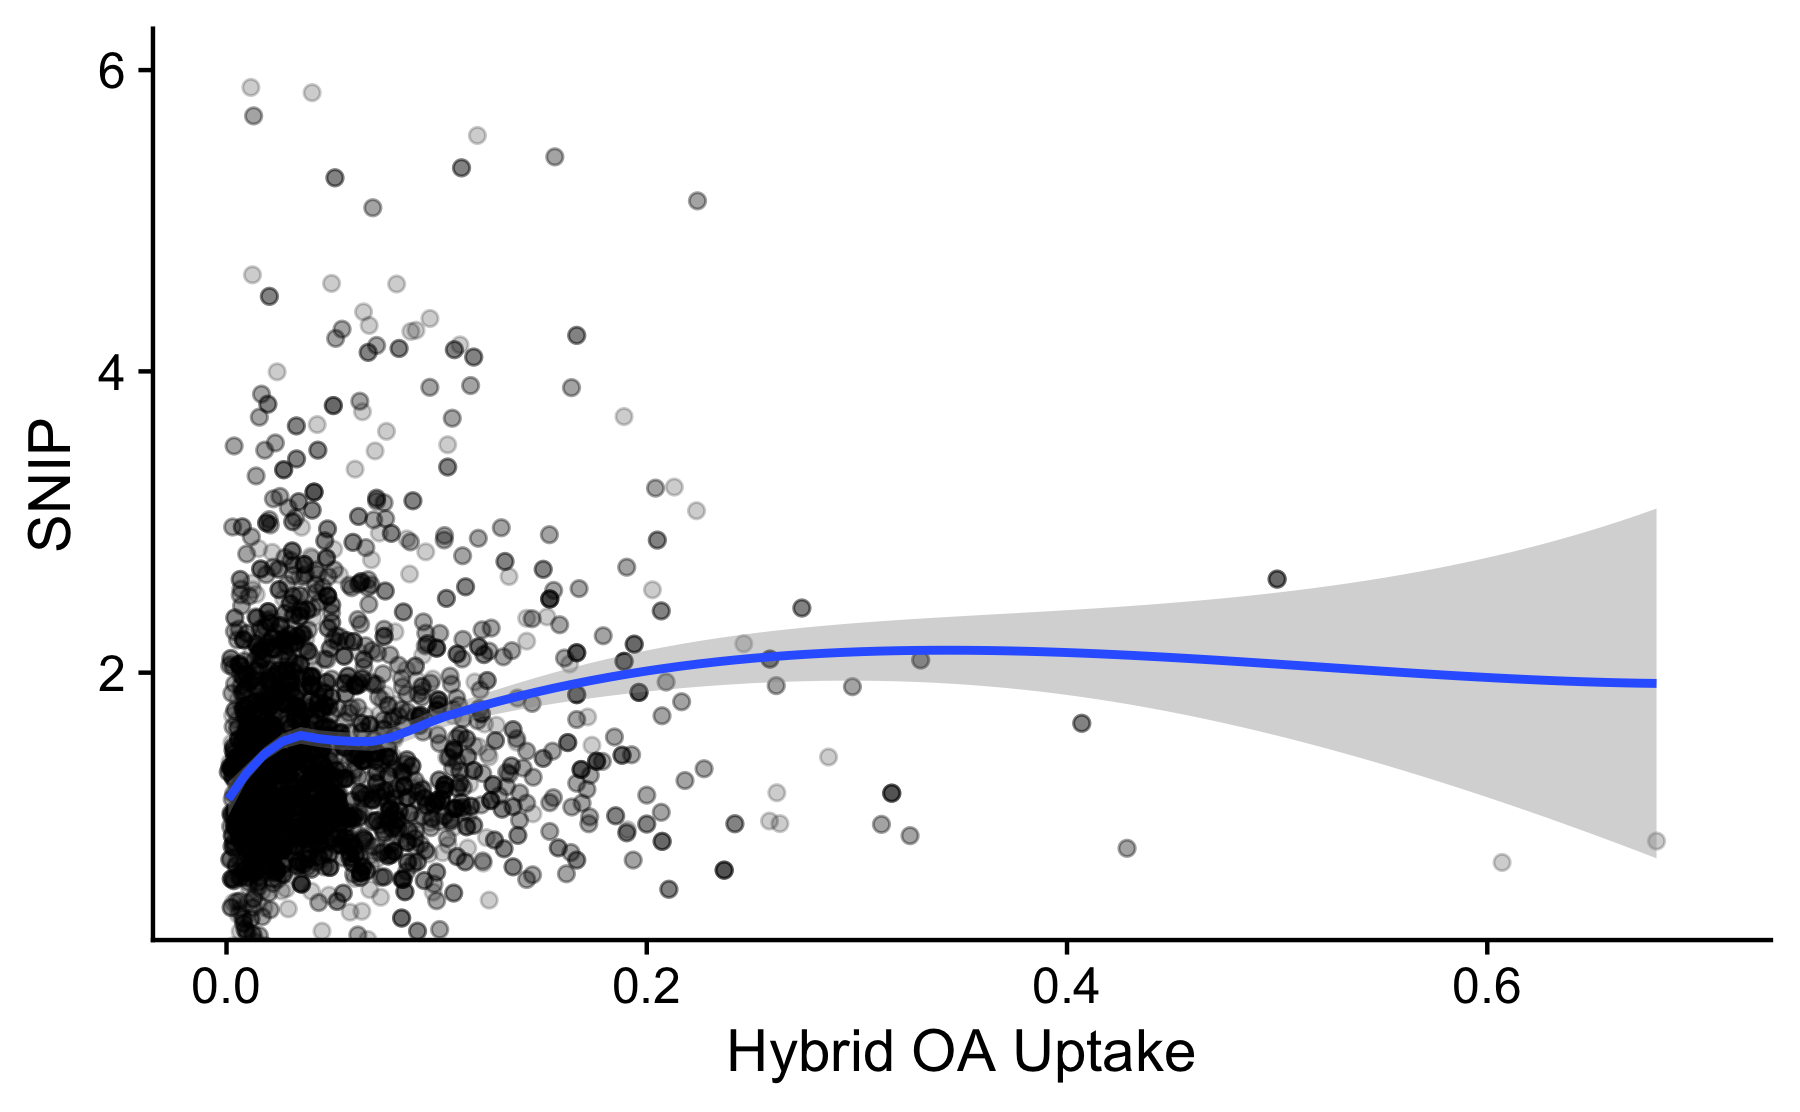
\includegraphics[width=0.7\linewidth,]{manuscript_files/figure-latex/sniptest-1} 

}

\caption{Source Normalized Impact per Paper (SNIP) versus open access (OA) uptake 2019. Each dot represents a hybrid journal with at least one published OA article in 2019. There is only a weak, positive correlation between the two variables ($r_s$=0.1679, $p<0.001$)}\label{fig:sniptest}
\end{figure}

\hypertarget{invoicing-for-hybrid-open-access}{%
\subsection*{Invoicing for Hybrid Open
Access}\label{invoicing-for-hybrid-open-access}}
\addcontentsline{toc}{subsection}{Invoicing for Hybrid Open Access}

\hypertarget{invoice-channels}{%
\subsubsection*{Invoice Channels}\label{invoice-channels}}
\addcontentsline{toc}{subsubsection}{Invoice Channels}

As can be seen from Table \ref{tab:invoicing_overview}, hybrid OA APC
were most often invoiced to authors (n=41,725; 58.2\%) and to a lesser
extent as part of agreements (n=24,250; 33.8\%). Interestingly, we also
found a small number of cases where hybrid APCs were waived (n=4,345;
6.1\%).

\begin{table}

\caption{\label{tab:invoicing_overview}Invoice channels for hybrid OA in Elsevier journals between 2015-19.}
\centering
\begin{tabular}[t]{lrr}
\toprule
Invoicing channel & Hybrid OA articles (n) & Percentage\\
\midrule
Author & 41,725 & 58.2\\
Agreement & 24,250 & 33.8\\
Fee waived & 4,345 & 6.1\\
Other & 1,323 & 1.8\\
\midrule
Total & 71,643 & 100.0\\
\bottomrule
\end{tabular}
\end{table}

Figure \ref{fig:invoiceoverview} illustrates that over the years,
Elsevier has increasingly invoiced hybrid OA APCs directly to authors
compared to research funders or academic consortia (``Agreement''). The
share of fee-waived articles remained relatively stable, but we found
different types of waivers. Around 51.7\% of fee waivers were linked to
an OA sponsor, which indicates that a third party paid the APC. For
instance, 853 waivers were linked to the French Académie des Sciences,
presumably covering OA publication in its society journals for
affiliated authors. The remaining 48.3\% of waived articles did not
disclose any OA sponsor. Moreover, Figure \ref{fig:invoiceoverview}
compares the invoicing channels based on open content license variants.
When Elsevier invoiced authors directly, most OA articles in hybrid
journals were published under a non-commercial license (n=32,086;
76.9\%), whereas most articles billed as part of agreements were
licensed under the more permissive CC BY license (n=18,331; 75.6\%).

\begin{figure}[H]

{\centering 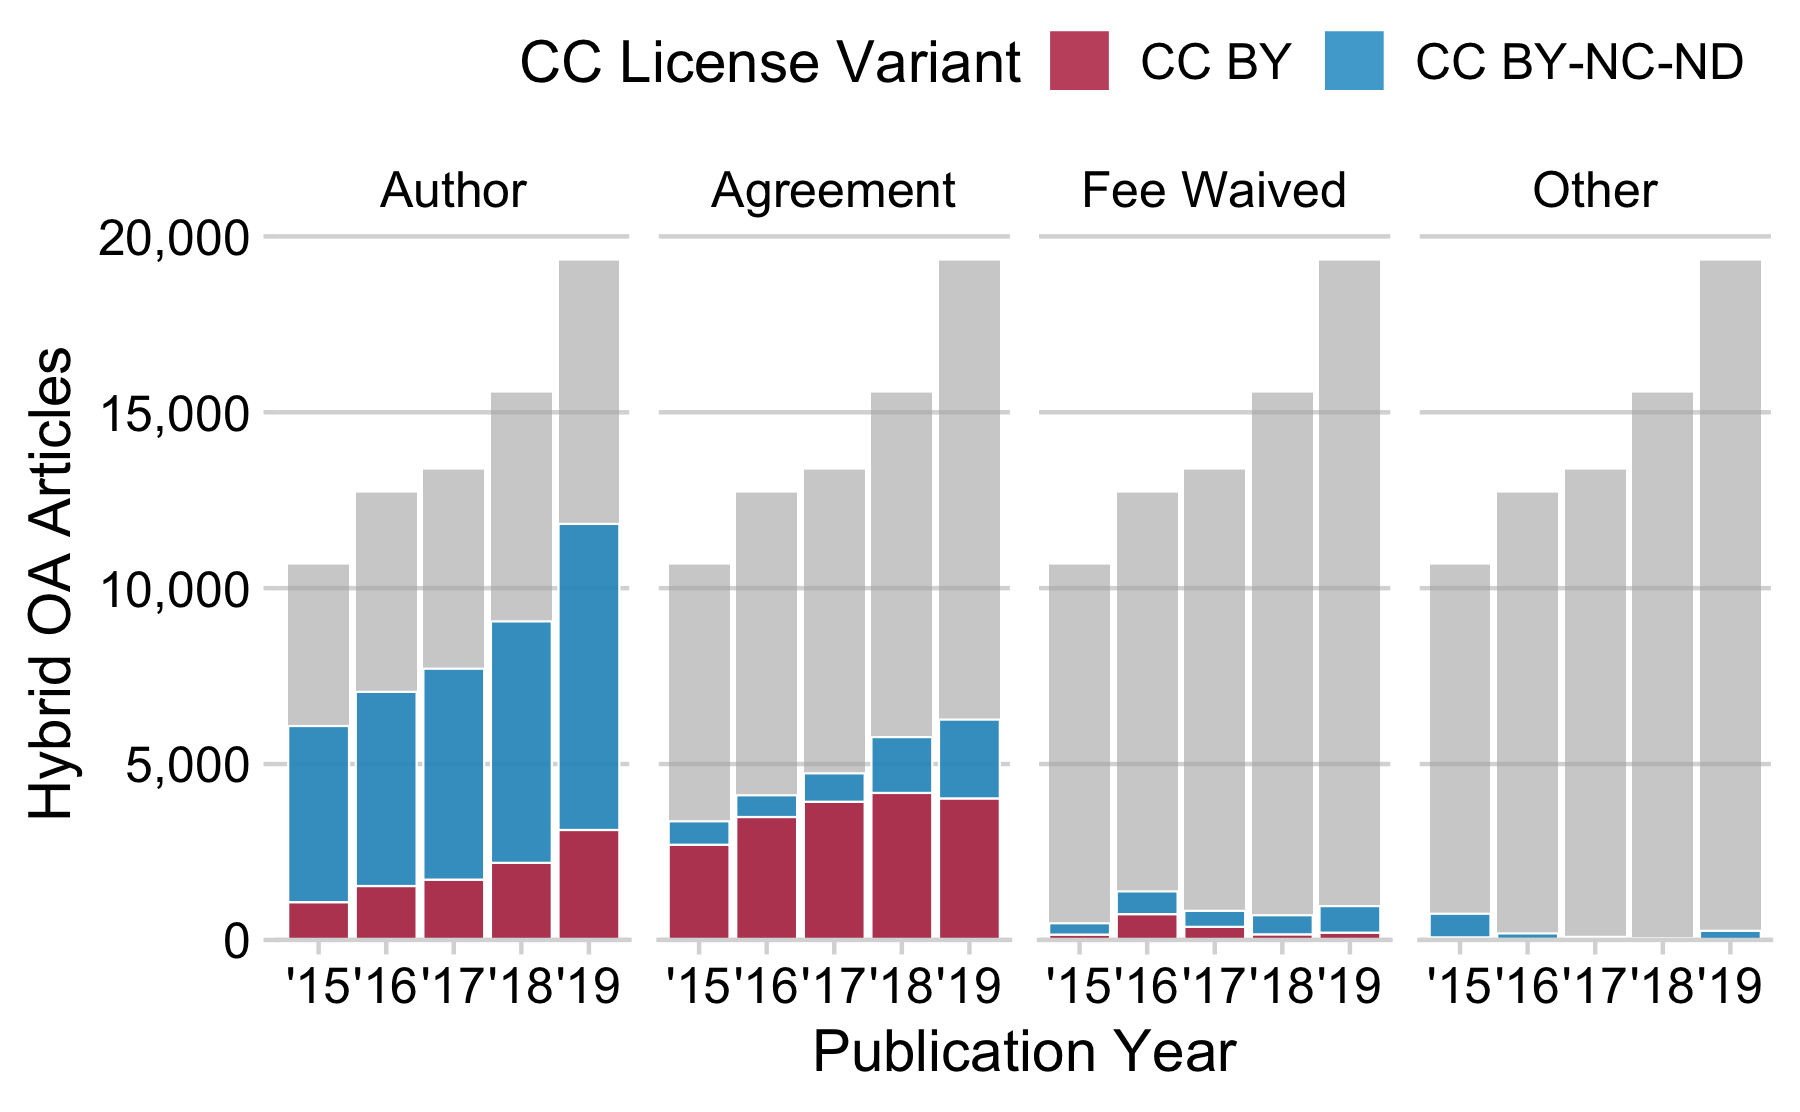
\includegraphics[width=0.7\linewidth,]{manuscript_files/figure-latex/invoiceoverview-1} 

}

\caption{Development of fee-based open access (OA) publishing in Elsevier hybrid journals by invoice channel Colored bars represent the share of OA articles invoiced to authors, agreements, or waived, grouped by Creative Commons license variant. Grey bars show the total number of hybrid OA articles published in Elsevier journals from 2015-2019.}\label{fig:invoiceoverview}
\end{figure}

We also observed large differences in OA invoicing among subject fields.
Table \ref{tab:invocing_by_subject} shows the number of OA articles by
subject field and invoice channel. For articles in nursing, decision
dciences, and pharmacology, toxicology and pharmaceutics, Elsevier
predominantly invoiced authors, whereas most energy and chemical
engineering articles were invoiced through agreements. Likewise, the
majority of articles in materials science, chemistry and physics and
astronomy were not invoiced to authors but facilitated through
agreements or waived. The large share of waived APCs in physics and
astronomy can be attributed to a single 2015 issue of Nuclear and
Particle Physics Proceedings, which offered sponsored OA.

\begin{table}[H]

\caption{\label{tab:invocing_by_subject}Invoice channels by discipline 2015-2019.}
\centering
\resizebox{\linewidth}{!}{
\begin{tabular}[t]{lrrrrr}
\toprule
\multicolumn{2}{c}{ } & \multicolumn{4}{c}{Invoice channel (in \%)} \\
\cmidrule(l{3pt}r{3pt}){3-6}
Subject & OA articles & Author & Agreement & Fee waived & Other\\
\midrule
Nursing & 1,504 & \cellcolor[HTML]{DC3977}{82} & \cellcolor[HTML]{FFFFFF}{16} & \cellcolor[HTML]{FFF7E8}{1} & \cellcolor[HTML]{FCDE9C}{1}\\
Decision Sciences & 785 & \cellcolor[HTML]{E6576F}{72} & \cellcolor[HTML]{FCC088}{27} & \cellcolor[HTML]{FFFFFF}{0} & \cellcolor[HTML]{FCDE9C}{1}\\
Pharmacology, Toxicology and Pharmaceutics & 4,075 & \cellcolor[HTML]{EA646F}{69} & \cellcolor[HTML]{FCC088}{27} & \cellcolor[HTML]{FFF7E8}{1} & \cellcolor[HTML]{FAA476}{2}\\
Business, Management and Accounting & 1,751 & \cellcolor[HTML]{EC686E}{68} & \cellcolor[HTML]{FBAF7D}{29} & \cellcolor[HTML]{FFF0D2}{2} & \cellcolor[HTML]{FCDE9C}{1}\\
Dentistry & 288 & \cellcolor[HTML]{EC686E}{68} & \cellcolor[HTML]{FFFAF1}{17} & \cellcolor[HTML]{F89774}{10} & \cellcolor[HTML]{DC3977}{5}\\
Health Professions & 674 & \cellcolor[HTML]{ED6D6E}{67} & \cellcolor[HTML]{FCD898}{24} & \cellcolor[HTML]{FFE8BB}{3} & \cellcolor[HTML]{DC3977}{5}\\
Medicine & 23,623 & \cellcolor[HTML]{F0756E}{65} & \cellcolor[HTML]{FCD092}{25} & \cellcolor[HTML]{FCC98E}{6} & \cellcolor[HTML]{E34F6F}{4}\\
Agricultural and Biological Sciences & 7,956 & \cellcolor[HTML]{F38170}{63} & \cellcolor[HTML]{F9A075}{31} & \cellcolor[HTML]{FCD697}{5} & \cellcolor[HTML]{FCDE9C}{1}\\
Computer Science & 3,185 & \cellcolor[HTML]{F38170}{63} & \cellcolor[HTML]{F27F70}{36} & \cellcolor[HTML]{FFFFFF}{0} & \cellcolor[HTML]{FCDE9C}{1}\\
Economics, Econometrics and Finance & 2,071 & \cellcolor[HTML]{F48771}{62} & \cellcolor[HTML]{F79373}{33} & \cellcolor[HTML]{FCD697}{5} & \cellcolor[HTML]{FFFFFF}{0}\\
Veterinary & 2,091 & \cellcolor[HTML]{F58D72}{61} & \cellcolor[HTML]{FCD092}{25} & \cellcolor[HTML]{F1766E}{13} & \cellcolor[HTML]{FCDE9C}{1}\\
Social Sciences & 6,306 & \cellcolor[HTML]{F79273}{60} & \cellcolor[HTML]{F27F70}{36} & \cellcolor[HTML]{FFE8BB}{3} & \cellcolor[HTML]{FFFFFF}{0}\\
Earth and Planetary Sciences & 4,532 & \cellcolor[HTML]{F89874}{59} & \cellcolor[HTML]{F48671}{35} & \cellcolor[HTML]{FCD697}{5} & \cellcolor[HTML]{FFFFFF}{0}\\
Biochemistry, Genetics and Molecular Biology & 15,903 & \cellcolor[HTML]{F89874}{59} & \cellcolor[HTML]{F48671}{35} & \cellcolor[HTML]{FDE1A5}{4} & \cellcolor[HTML]{FAA476}{2}\\
Immunology and Microbiology & 5,542 & \cellcolor[HTML]{F89874}{59} & \cellcolor[HTML]{F58D72}{34} & \cellcolor[HTML]{FCC98E}{6} & \cellcolor[HTML]{FAA476}{2}\\
Environmental Science & 9,000 & \cellcolor[HTML]{F99D75}{58} & \cellcolor[HTML]{EF726E}{38} & \cellcolor[HTML]{FFE8BB}{3} & \cellcolor[HTML]{FCDE9C}{1}\\
Psychology & 3,087 & \cellcolor[HTML]{FAA376}{57} & \cellcolor[HTML]{EC686E}{40} & \cellcolor[HTML]{FFF0D2}{2} & \cellcolor[HTML]{FCDE9C}{1}\\
Neuroscience & 5,906 & \cellcolor[HTML]{FBAA7A}{56} & \cellcolor[HTML]{EC686E}{40} & \cellcolor[HTML]{FFE8BB}{3} & \cellcolor[HTML]{FCDE9C}{1}\\
Arts and Humanities & 1,565 & \cellcolor[HTML]{FCB882}{54} & \cellcolor[HTML]{E4536F}{44} & \cellcolor[HTML]{FFF7E8}{1} & \cellcolor[HTML]{FFFFFF}{0}\\
Mathematics & 2,105 & \cellcolor[HTML]{FCBF87}{53} & \cellcolor[HTML]{EF726E}{38} & \cellcolor[HTML]{FBAF7D}{8} & \cellcolor[HTML]{FFFFFF}{0}\\
Engineering & 8,405 & \cellcolor[HTML]{FCD395}{50} & \cellcolor[HTML]{E24C70}{46} & \cellcolor[HTML]{FFE8BB}{3} & \cellcolor[HTML]{FCDE9C}{1}\\
Materials Science & 4,838 & \cellcolor[HTML]{FCDA99}{49} & \cellcolor[HTML]{E14971}{47} & \cellcolor[HTML]{FDE1A5}{4} & \cellcolor[HTML]{FFFFFF}{0}\\
Chemistry & 4,033 & \cellcolor[HTML]{FCE0A1}{48} & \cellcolor[HTML]{E24C70}{46} & \cellcolor[HTML]{FCD697}{5} & \cellcolor[HTML]{FCDE9C}{1}\\
Energy & 4,286 & \cellcolor[HTML]{FEE7B8}{46} & \cellcolor[HTML]{DC3977}{52} & \cellcolor[HTML]{FFF7E8}{1} & \cellcolor[HTML]{FCDE9C}{1}\\
Chemical Engineering & 2,977 & \cellcolor[HTML]{FFEBC4}{45} & \cellcolor[HTML]{E14971}{47} & \cellcolor[HTML]{FCBC85}{7} & \cellcolor[HTML]{FCDE9C}{1}\\
Physics and Astronomy & 5,859 & \cellcolor[HTML]{FFFFFF}{40} & \cellcolor[HTML]{EF726E}{38} & \cellcolor[HTML]{DC3977}{22} & \cellcolor[HTML]{FFFFFF}{0}\\
\bottomrule
\end{tabular}}
\end{table}

\hypertarget{invoice-recipients}{%
\subsubsection*{Invoice Recipients}\label{invoice-recipients}}
\addcontentsline{toc}{subsubsection}{Invoice Recipients}

Elsevier's data offer more insight into invoicing. Overall, we
identified 62 sponsoring institutions and organizations that received
invoices for hybrid publishing fees as part of an agreement with
Elsevier. We found that, by a large margin, most invoices were issued to
UK-based research funders and institutions (n=14,344; 59.2\%), followed
by the Netherlands (n=2,835; 11.7\%) and the European Union (n=2,164;
8.9\%; EU). Figure \ref{fig:invoice_sponsor_country} provides a closer
look at the geographical distribution by license prevalence,
highlighting the dominance of CC -BY licensed articles invoiced to
sponsoring institutions in the UK, the United States, and, to a much
lesser extent, the Netherlands. In contrast, the majority of articles
invoiced to sponsoring institutions from Norway or representing the EU
were published under a non-commercial license.

\begin{figure}[H]

{\centering 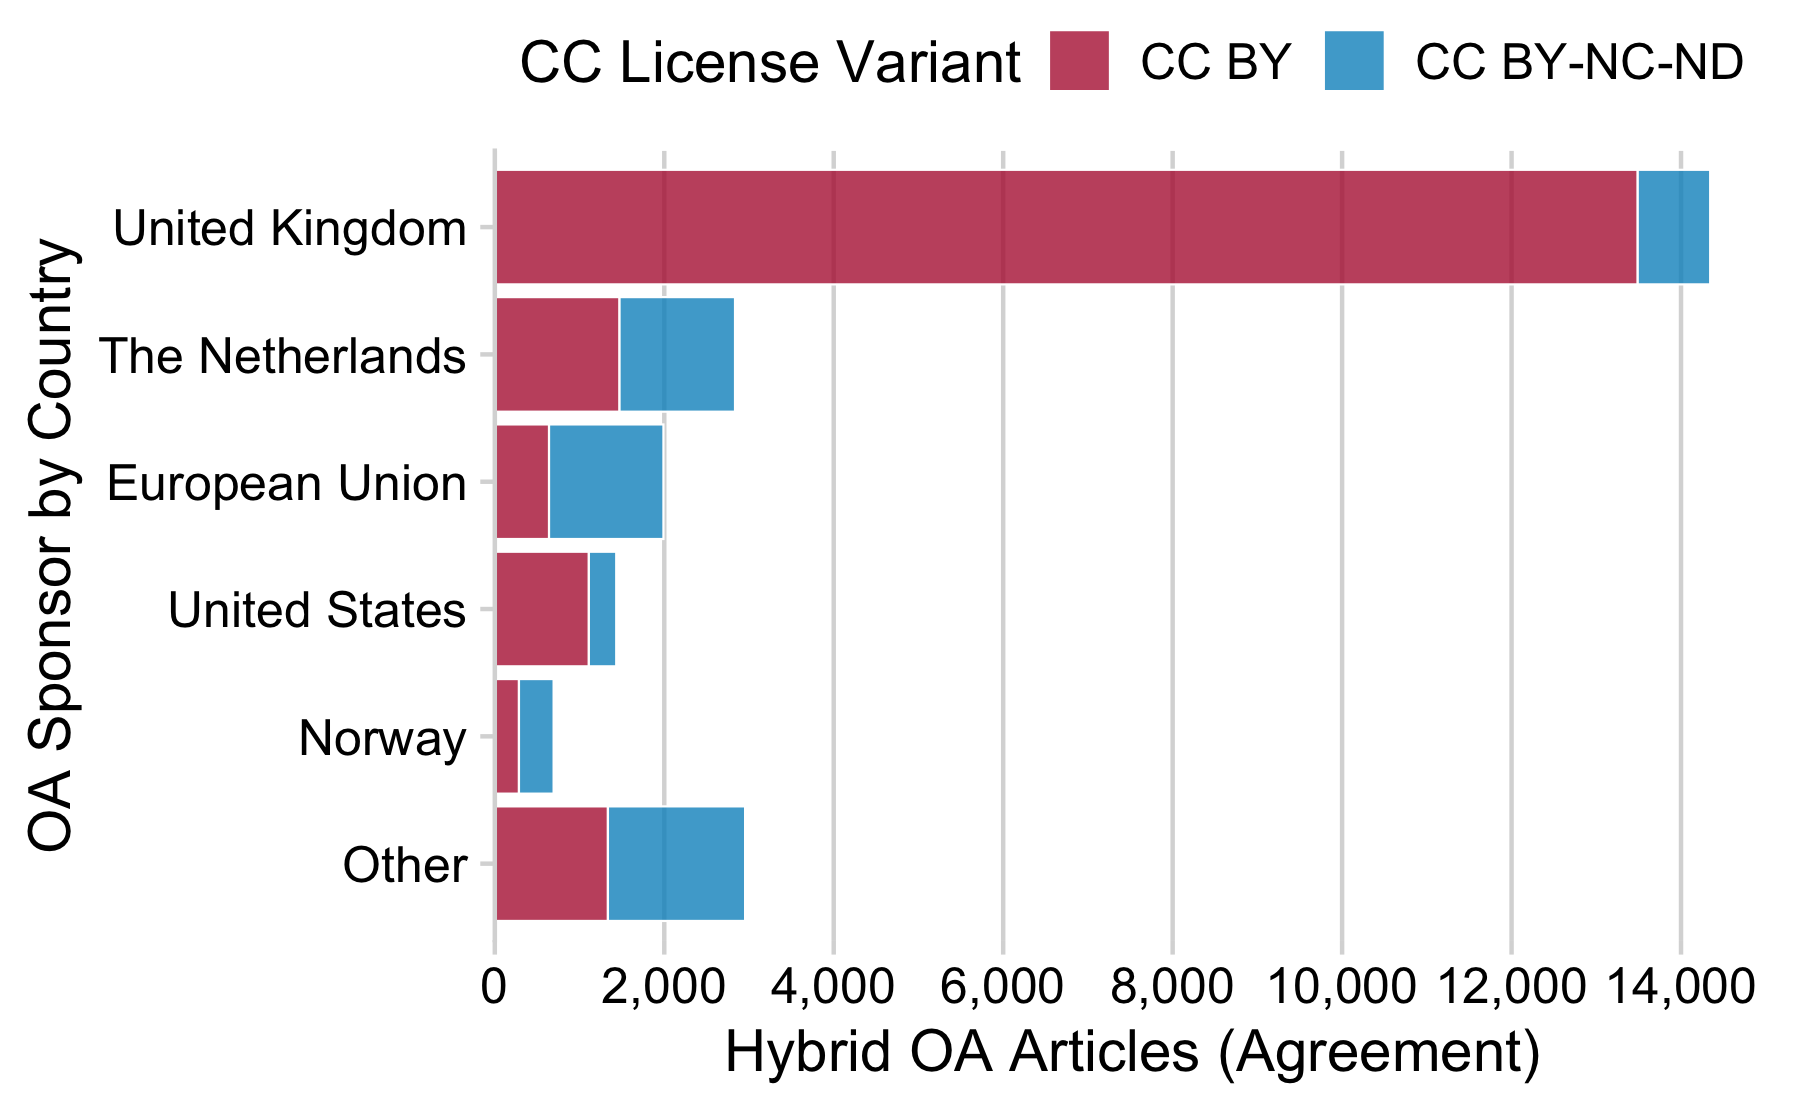
\includegraphics[width=0.7\linewidth,]{manuscript_files/figure-latex/invoice_sponsor_country-1} 

}

\caption{Number of centrally invoiced OA articles in Elsevier hybrid journals by country of recipient. Colored bars represent the Creative Commons (CC) license variant under which the article was published between 2015 and 2019.}\label{fig:invoice_sponsor_country}
\end{figure}

Figure \ref{fig:sponsor_sector} shows the yearly distribution of central
invoiced articles by year and institutional sector. While UK-based OA
invoices were mainly addressed to discipline-specific governmental and
non-profit research funders, invoices to the Netherlands and Norway were
issued to national academic consortia representing the higher education
sector. In 2019, Elsevier also launched similar agreements in countries
with lower publication output including Hungary and Poland. Besides, we
found that invoiced funding bodies from the UK and the US mainly
represented discipline-specific funders, while the invoiced funding
bodies from other countries were focused on a broad variety of
disciplines (see Table \ref{tab:subject_profile}).

\begin{figure}[H]

{\centering 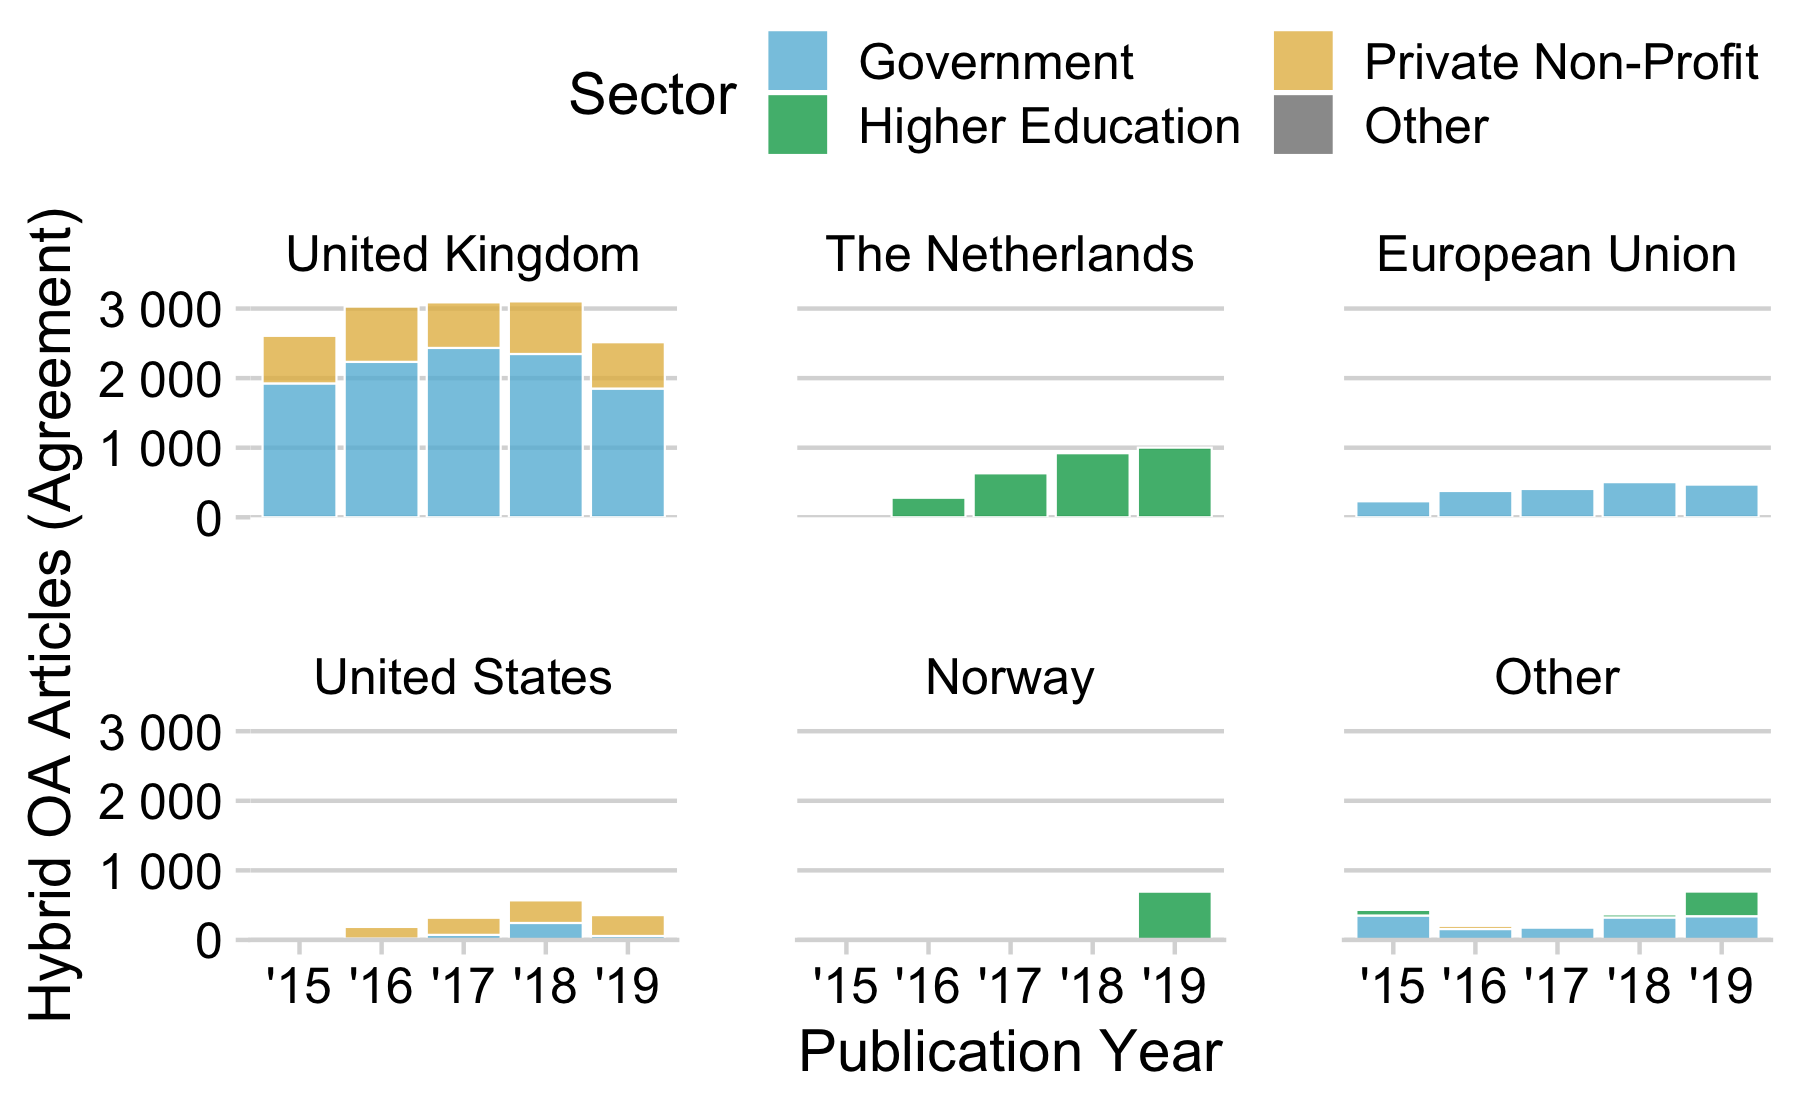
\includegraphics[width=0.7\linewidth,]{manuscript_files/figure-latex/sponsor_sector-1} 

}

\caption{ Development of centrally invoiced OA articles in hybrid journals by country. Colored bars represent the institutional sector OA funding bodies belong to.}\label{fig:sponsor_sector}
\end{figure}

\begin{table}

\caption{\label{tab:subject_profile} Relative subject profile of centrally invoiced OA funding bodies.}
\centering
\resizebox{\linewidth}{!}{
\begin{tabular}[t]{l|rrrrr|rl|rrrrr|rl|rrrrr|rl|rrrrr|rl|rrrrr|rl|rrrrr|rl|rrrrr|r}
\toprule
Country/Subject area & Health science & Life sciences & Physical sciences & SSH & Broad & Total\\
\midrule
United Kingdom & 25\% & 11\% & 21\% & 5\% & 0\% & 62\%\\
The Netherlands & 0\% & 0\% & 0\% & 0\% & 12\% & 12\%\\
European Union & 0\% & 0\% & 0\% & 0\% & 9\% & 9\%\\
United States & 6\% & 0\% & 0\% & 0\% & 1\% & 7\%\\
Norway & 0\% & 0\% & 0\% & 0\% & 3\% & 3\%\\
\addlinespace
Other & 1\% & 0\% & 1\% & 0\% & 5\% & 7\%\\
\midrule
Total & 32\% & 11\% & 22\% & 5\% & 30\% & 100\%\\
\midrule
\bottomrule
\end{tabular}}
\end{table}

\hypertarget{institutional-ranking}{%
\subsubsection*{Institutional ranking}\label{institutional-ranking}}
\addcontentsline{toc}{subsubsection}{Institutional ranking}

Table \ref{tab:sponsor_top_10} presents the top ten of 63 sponsoring
bodies in our sample. Together, they accounted for around 80\% of
centrally invoiced APCs. The table also highlights the number of
distinct journals and the share of CC BY licensed articles. Notably,
UK-based research funders and the US-based Bill and Melinda Gates
Foundation mainly sponsored articles published under a CC BY license. In
contrast, articles funded by VSNU, the European Research Council, and
Norway Institutes had a much lower proportion of CC BY.

\begin{table}

\caption{\label{tab:sponsor_top_10} Top 10 Elsevier hybrid OA sponsors by centrally invoiced articles 2015-2019.  The table furthermore presents the number of Elsevier hybrid journals with at least one invoiced article and two indicators of compliance: proportion of  CC BY licensed articles  and disclosed spending through the Open APC Initiative (OAPC.}
\centering
\resizebox{\linewidth}{!}{
\begin{tabular}[t]{lrrrrr}
\toprule
\multicolumn{4}{c}{ } & \multicolumn{2}{c}{Compliance (in \%)} \\
\cmidrule(l{3pt}r{3pt}){5-6}
Hybrid OA sponsors & Journals & Articles & \% & CC BY & OAPC\\
\midrule
Engineering and Physical Sciences Research Council & 619 & 4663 & 19 & \cellcolor[HTML]{DE3E75}{97} & \cellcolor[HTML]{E34E6F}{55}\\
VSNU & 357 & 2835 & 12 & \cellcolor[HTML]{FCC38A}{52} & \cellcolor[HTML]{FFFFFF}{0}\\
Wellcome Trust & 448 & 2506 & 10 & \cellcolor[HTML]{DD3D76}{98} & \cellcolor[HTML]{DD3D76}{66}\\
European Research Council & 541 & 1986 & 8 & \cellcolor[HTML]{FFFFFF}{32} & \cellcolor[HTML]{FFE9BD}{9}\\
Medical Research Council & 384 & 1922 & 8 & \cellcolor[HTML]{DF4274}{95} & \cellcolor[HTML]{E6596F}{51}\\
Natural Environment Research Council & 203 & 1357 & 6 & \cellcolor[HTML]{DE3E75}{97} & \cellcolor[HTML]{EC696E}{45}\\
Biotechnology and Biological Sciences Research Council & 309 & 1169 & 5 & \cellcolor[HTML]{E04573}{93} & \cellcolor[HTML]{F0736E}{41}\\
Bill and Melinda Gates Foundation & 254 & 1030 & 4 & \cellcolor[HTML]{DC3977}{100} & \cellcolor[HTML]{DC3977}{68}\\
Economic and Social Research Council & 245 & 922 & 4 & \cellcolor[HTML]{DE4075}{96} & \cellcolor[HTML]{E9616F}{48}\\
Norway Institutes & 374 & 694 & 3 & \cellcolor[HTML]{FFE9BD}{41} & \cellcolor[HTML]{FFFFFF}{0}\\
Other & 1012 & 5166 & 21 & \cellcolor[HTML]{FCBA84}{54} & \cellcolor[HTML]{FCBF87}{21}\\
\midrule
All & 1423 & 24250 & 100 & \cellcolor[HTML]{ED6C6E}{76} & \cellcolor[HTML]{F48671}{36}\\
\midrule
\bottomrule
\end{tabular}}
\end{table}

The table also highlights the proportion of APC funding publicly
disclosed through the Open APC initiative, showing higher disclosure
rates for funders with a large CC BY share. On the other hand, APCs that
were invoiced as part of transformative agreements were not publicly
shared.

Figure \ref{fig:field_funder_matrix} shows the subject profile of OA
sponsors based on to the journals' subject fields of centrally invoiced
articles. As expected, the figure shows that subject-specific funders,
such as the British Engineering and Physical Sciences Research Council
(EPSRC), tended to focus on a limited set of subject fields. In
contrast, national consortia, such as VSNU and Norwegian Institutes
(NO), financed OA articles for a broader range of fields. However,
within these consortia, the subject distribution also varied. VSNU OA
spending, for example, had a strong focus on articles relating to
medicine, environmental science, and energy, presumably reflecting
disciplines with a generally strong publication output at Dutch
universities. Norwegian universities mostly published hybrid OA in
engineering, environmental science and agricultural and biological
sciences journals.

\begin{figure}[H]

{\centering 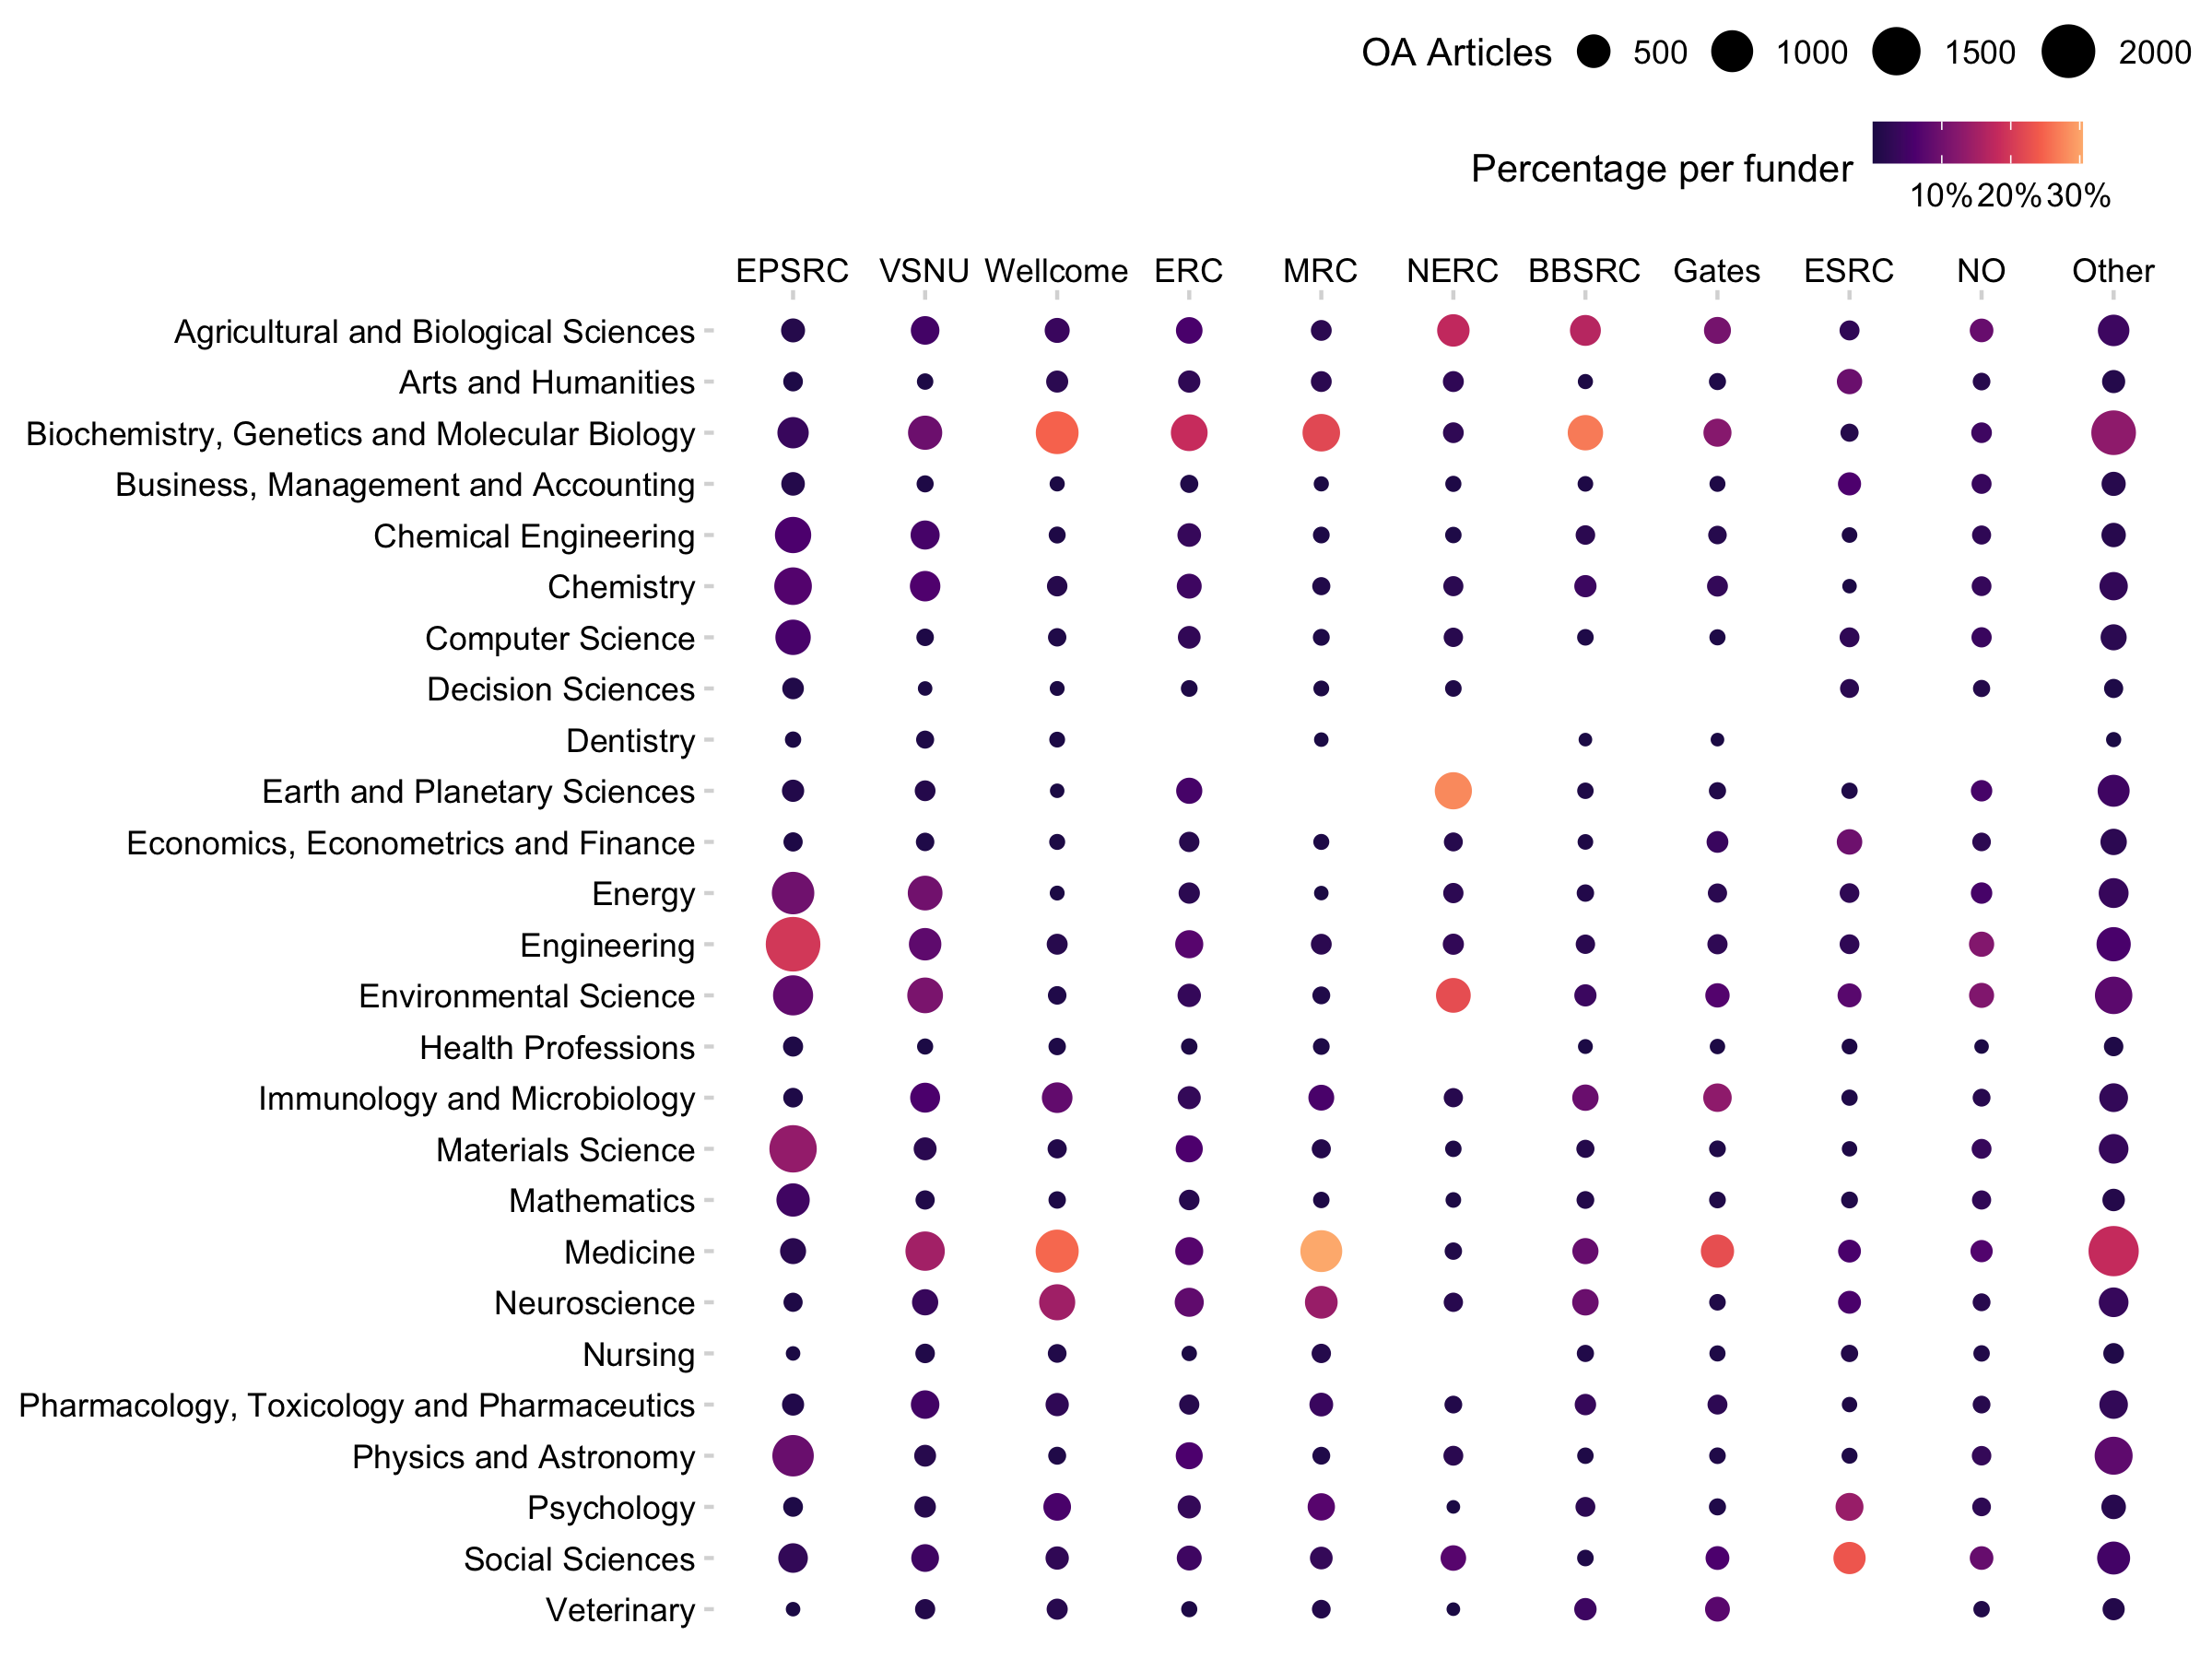
\includegraphics[width=0.95\textwidth]{../figure/funder_subject.png}

}

\caption{Top 10 Elsevier hybrid OA institutional invoice recipients in terms of articles published by journal subject. EPSRC, Engineering and Physical Sciences Research Council; VSNU, VSNU; Wellcome, Wellcome Trust; ERC, European Research Council; ERC, European Research Council; MRC, Medical Research Council; NERC, Natural Environment Research Council; BBSRC, Biotechnology and Biological Sciences Research Council; Gates, Bill and Melinda Gates Foundation; ESRC, Economic and Social Research Council; NO, Norway Institutes. }\label{fig:field_funder_matrix}
\end{figure}

\hypertarget{discussion}{%
\section{Discussion}\label{discussion}}

Over the last five years, Elsevier recorded growth in the uptake of
hybrid OA for each of our three indicators: The number of hybrid OA
articles published per year doubled, the number of hybrid journals with
at least one OA article grew by 21\%, and the share of hybrid OA
articles relative to closed-accessed articles in these journals
increased from 2.6\% to 3.7\%. As Laakso \& Björk (2016), we found only
a weak relationship between citation metrics like the SNIP and hybrid OA
uptake and observed differences in the uptake of hybrid OA among journal
subject areas. In particular, we found the highest count of hybrid OA
articles in physical sciences journals (see Table
\ref{tab:subject_area_table}). This was followed by the life sciences
and health sciences, whereas the social sciences had the lowest count of
hybrid articles. This order mostly reflects the disciplines' overall
publication output. According to the Open Science Monitor by the
European Commission, the physical sciences and mathematics publish the
most articles, followed by the health sciences, life sciences, and
social sciences and humanities.

Such disciplinary differences in hybrid OA prevalence become more
meaningful when considering the relative share of OA articles to
closed-access articles. In line with previous research, we found that
Elsevier journals from the life sciences and social sciences (Jubb et
al., 2017; Kramer \& Bosman, 2018; Laakso \& Björk, 2016) recorded
greater than typical hybrid OA uptake, whereas physical sciences
journals generally had a lower than typical uptake (Kramer \& Bosman,
2018; Laakso \& Björk, 2016; Martín-Martín et al., 2018). In a
systematic review of OA publishing patterns, Severin et al. (2020)
linked such disciplinary differences to socio-cultural and technological
factors that shape publishing cultures and practices. Among other
aspects, the authors pointed to the availability of prestigious
journals, the possibility to provide OA through alternative routes, and
ease of access to funding sources to cover publishing fees. As such,
looking at hybrid OA uptake in isolation can only provide limited
insight, so that placing it within the broader context of disciplinary
publishing and OA practices is necessary. For instance, since many
branches of the physical sciences have established self-archiving
practices and the technical infrastructure to support these (e.g., the
arXiv; Severin et al. (2020), Björk et al. (2010), Laakso \& Björk
(2016)), researchers can provide OA through repositories (i.e., green
OA), and indeed, according to the Open Science Monitor the physical
sciences provide OA primarily through the green route (31.2\% total OA
share, 24\% OA if only considering green OA). Hence, the low share of
hybrid OA in our sample might be because physical scientists perceive
much less of a need for hybrid OA. Further, Severin et al. (2020) note
project-based funding structures enable OA publishing in fully OA and
hybrid journals as they allow for easy integration of publishing costs.
Since these funding structures are typical for the life sciences
(ibid.), we would expect higher rates of OA. Data from the Open Science
Monitor seems to support this notion as the life sciences record
particularly high shares of full OA articles and comparatively high
shares of hybrid OA in some fields, such as biology and agricultural
science. While we expected the observed hybrid OA shares for the life
sciences and physical sciences, we were surprised by the high share of
hybrid OA belonging to the AJSC subject area social sciences, which also
includes the humanities, since articles ``social scientists have
reported to face significant difficulties in access to grant funding for
{[}publication charges{]}, as most research in the social sciences is
not done by means of project-specific funding'' Severin et al. (2020, p.
15). However, previous research has found comparatively low awareness
and uptake of green OA among researchers in the field (Björk et al.,
2010; Creaser et al., 2010), which might encourage hybrid OA uptake.
Another possible explanation,is that Elsevier has a number of high
prestigious social science and humanities journals (Larivière et al.,
2015), which means that our findings are not representative of the
general population of SSH journals. Likewise, this limitation could be
extended to our findings in general that whilst not representative of
the population of hybrid OA publishing, they provide valuable insight
into a key player of scholarly publishing.

Finally, OA policies in favor of hybrid OA in combination with invoicing
agreements with Elsevier might be a driver. For instance, we found that
nearly half of articles in arts and humanities were facilitated through
agreements, which was above-average. This is in line with previous
research, suggesting that OA policies and funder mandates have a
stronger effect on OA uptake than disciplinary publication cultures
(Huang et al., 2020; Larivière \& Sugimoto, 2018).

Our overall investigation of invoice channels and recipients of hybrid
OA APCs found that the majority of Elsevier hybrid articles were
invoiced to the author (n=41,725; 58.2\%). However, it is important to
note that although Elsevier's metadata classifies the sponsor type as
``author'', this does not necessarily mean that authors paid for APCs
out of their own pocket but rather just that the APC was not invoiced
through an agreement. Hence, it is possible that APCs invoiced to the
author were covered by institutional funds or as part of research
grants. For instance, a recent Springer Nature survey found that hybrid
OA was predominantly supported through institutional and funder sources
(71\%), followed by OA agreements (34\%), while only 6\% were paid from
personal funds or savings (Monaghan et al., 2020). We also observed
notable differences in licensing among invoice types. The majority of
hybrid OA articles, regardless of the invoice type, were licensed under
the more restrictive CC BY-NC-ND license. There is a lack of dedicated
studies on licence selection, but indications so far suggest that when
given a choice authors tend to select more restrictive variants for
their published works (Fraser et al., 2020; Noorden, 2013; Rowley et
al., 2017). On the other hand, when hybrid articles were invoiced
through agreements, most articles were licensed under the more liberal
CC BY license. As several funding bodies mandate CC BY licenses,
including the UK research funders that account for 62\% of our
``agreement'' subsample, this result is perhaps not surprising but
suggests the effectiveness of such agreements.

Based on our findings, around a third of the articles were invoiced
directly through OA agreements (e.g., research funders, national library
consortia). Strikingly, sponsors based in the UK accounted for more than
half of these , and a quarter was charged to sponsors from other
European countries. This finding reiterates reports from previous
studies that the UK's OA profile differs markedly from other countries
(cf.~ref, ref) and points to the effects of science policy. To increase
OA to research publications, the UK implemented centralized APC funding
and embraced hybrid OA as a transition model. Within five years of the
publication of the Finch Report in 2012, the UK recorded an 18\%
increase in immediate OA, coupled with a rise in hybrid OA from 2.7\% in
2012 to 15.4\% of all articles in 2016 (Jubb et al., 2017), which can be
attributed to the availability of APC funding from Research Councils UK
(RCUK). Indeed, RCUK block grants have been the largest single source of
OA funds in the UK---the Wellcome Trust, and more recently
transformative agreements (Jubb et al., 2017; Tickel, 2018). However,
since then publishing expenditures of UK universities have been rising
rapidly (ref), so that several universities stopped supporting hybrid OA
in late 2018-2019 (Castro, 2019; University of Birmingham, n.d.;
University of Oxford, 2019; Walker, 2019). This development might
explain the slight decrease in hybrid articles invoiced to the UK our
data showed around that time (see Figure
\ref{fig:invoice_sponsor_country}).

An essential part in the absence of transparency in scholarly publishing
and especially in hybrid OA has been the lack of transparency in
publishers' article management. This has prohibited consumers to get a
comprehensive and comparative overview of their publishing activities
and the associated costs and, thus, limited their negotiating power.
However, certain initiatives in Europe like the ESAC Initiative have
begun to press for improved and more transparent workflows for
transformative agreements (Geschuhn \& Stone, 2017). In particular, the
ESAC Workflow Recommendations seek to increase efficiency and
transparency in the publication workflow through improved invoicing and
reporting processes and metadata delivery, including article-based
machine readable information about the OA sponsor. Through this study we
demonstrated the utility and benefits of such publisher-provided
metadata about hybrid OA funding and highlighted the need for extending
these to include comprehensive information about the licensing and the
particular OA type.

Usually identifying delayed OA articles and distinguishing them from
other types of OA is challenging since there is no publicly available
list of such journals. For instance, Taylor \& Francis' (2021) website
indicates that some of their journals participate in a delayed or
promotional OA program but no further information is provided as to
which journals these are. However, Elsevier provides a list of journals
enrolled in the ``Open Archive'' programme and further tags delayed OA
articles in the machine-readable XML version of the article. This
enables easy identification and more accurate assessments of hybrid OA,
which allows to take into account the substantial amount of delayed OA
content in future hybrid OA studies using Elsevier data.

While this study advances our knowledge about hybrid OA uptake and
invoicing, the limitations leave room for future research. This study
focused on only one publisher, which limits the generalizability of our
findings since Elsevier's attributes such as composition of the journal
portfolio, mix of business models, pricing, and promotion of various
options cannot be assumed to be representative of scholarly journal
publishing in general. Though the invoicing data extracted from the XML
files enables unprecedented accuracy and comprehensiveness in the study
of hybrid OA, it likely does not disclose the actual OA sponsor in all
cases. Most articles were invoiced to authors, but it remains unclear
how often authors themselves pay for APCs or invoices are covered
through institutional OA funds or research grants. Further research into
this topic would increase our understanding of OA funding streams
outside of publishing agreements. Further, our study demonstrates that
to achieve comprehensive mapping and understanding of the financial
flows involved in OA funding, complex, in-depth country-specific
meso-level analyses is needed. Such studies would ideally draw on
various data sources, such as publicly available bibliometrics and
metadata, information about significant national research funders and
their OA policies, information about the national library and possible
consortia landscape including their publishing agreements, which might
require Freedom of Information Requests.

This study provides a snapshot of hybrid OA for the largest journal
publisher prior to the impact of the implementation of Plan S
requirements. While many Plan S signatories have already had strong OA
policies, this harmonized approach is likely to affect publishing
decisions of funded authors,the licencing of their articles, and the
offerings and pricing of publishers. Since the new requirements are
applicable to research funded from 2021 onwards, a comparative study
focused on articles invoiced to Plan S signatories would be a fruitful
endeavor.

In a similar vein, future studies could combine invoice information with
research funding information since these contribute different pieces to
the funding stream puzzle. This could also provide more insight into the
actual APC funding streams behind the author-invoiced articles.

\hypertarget{conclusion}{%
\section{Conclusion}\label{conclusion}}

The primary aim of this empirical study was to investigate Elsevier's
hybrid OA publishing from 2015-2019 to better understand the volume and
invoicing of hybrid OA and present a novel, data-driven approach for
such analyses. Our results indicate that although the number of hybrid
OA articles has increased over time, hybrid OA uptake has remained low.
Notably, hybrid APCs were most often invoiced directly to the authors or
through institutional agreements, where only a few funding bodies were
the main driver of hybrid OA. Finally, our findings highlight that
publisher-provided metadata about the invoicing channels of (hybrid) OA
can facilitate research into and increase the understanding of the
financial flows of OA publishing.

Ever since its inception, hybrid OA has been a challenging subject to
study due to the lack of standardised ways for publishers to flag such
content and APC funding data being limited to studies based on surveys
and articles' acknowledgements sections. This study presented a novel
approach to studying OA APC invoicing that is based on publicly
available publisher-provided metadata, which can be used on on its own
or in combination with other public data sources to gain more detailed
and comprehensive insights into hybrid OA uptake and invoicing than ever
before. If more publishers reported OA invoicing data on the article
level and in a machine-readable format, this would increase transparency
and enable enhanced monitoring of the scholarly journal landscape over
time. As hybrid OA has increasingly become a central element of OA
policies of research funders and libraries, customer organisations could
require that invoicing information is added to the article-level
metadata. As long as publishers do not provide this data in a structured
and comprehensive format, they prevent consumers from benchmarking
prices and therefore hinder price competition as the only alternative to
gain comparative insight is self-reported APC expenditures that research
funders and libraries voluntarily report to the Open APC initiative. The
Open APC initiative is a valuable service but it cannot replace
publisher-provided data since global participation is limited.

From recent science policy developments in Europe it appears that Big
Deals have gained support and remain firmly in place in the form of
transformative agreements. However, in addition to research funders and
libraries that increasingly make publishing contracts public, it is on
the publisher to provide metadata as presented here to improve the
transparency in scholarly publishing by linking invoicing data to
bibliometrics. From this study we can affirm that hybrid OA is complex
as the financial flows come from various stakeholders and invoicing
forms, it is not just libraries or consortia, but authors and funders
are also directly involved. As of right now, providing machine-readable
article-level invoicing data is not common amongst publishers, which
limits the potential for broader studies.

\hypertarget{data-availability}{%
\section{Data Availability}\label{data-availability}}

All data and code used for this study is openly available on GitHub,
including version history:

\url{https://github.com/njahn82/elsevier_hybrid_invoicing}

Formal analyis is written in R Markdown and thus replicable.

\hypertarget{references}{%
\section*{References}\label{references}}
\addcontentsline{toc}{section}{References}

\hypertarget{refs}{}
\begin{cslreferences}
\leavevmode\hypertarget{ref-Akbaritabar_2019}{}%
Akbaritabar, A., \& Stahlschmidt, S. (2019). \emph{Applying crossref and
unpaywall information to identify gold, hidden gold, hybrid and delayed
open access publications in the KB publication corpus}. SocArXiv.
\url{https://doi.org/10.31235/osf.io/sdzft}

\leavevmode\hypertarget{ref-antelmann_2017}{}%
Antelman, K. (2017). Leveraging the growth of open access in library
collection decision making. \emph{At the helm: leading transformation},
411--422.

\leavevmode\hypertarget{ref-Bergstrom_2014}{}%
Bergstrom, T. C., Courant, P. N., McAfee, R. P., \& Williams, M. A.
(2014). Evaluating big deal journal bundles. \emph{Proceedings of the
National Academy of Sciences}, \emph{111}(26), 9425--9430.
\url{https://doi.org/10.1073/pnas.1403006111}

\leavevmode\hypertarget{ref-Bj_rk_2012}{}%
Björk, B.-C. (2012). The hybrid model for open access publication of
scholarly articles: A failed experiment? \emph{Journal of the American
Society for Information Science and Technology}, \emph{63}(8),
1496--1504. \url{https://doi.org/10.1002/asi.22709}

\leavevmode\hypertarget{ref-Bj_rk_2010}{}%
Björk, B.-C., Welling, P., Laakso, M., Majlender, P., Hedlund, T., \&
Guðnason, G. (2010). Open access to the scientific journal literature:
Situation 2009. \emph{PLoS ONE}, \emph{5}(6), e11273.
\url{https://doi.org/10.1371/journal.pone.0011273}

\leavevmode\hypertarget{ref-Borrego_2020}{}%
Borrego, Á., Anglada, L., \& Abadal, E. (2020). Transformative
agreements: Do they pave the way to open access? \emph{Learned
Publishing}. \url{https://doi.org/10.1002/leap.1347}

\leavevmode\hypertarget{ref-Castro_2019}{}%
Castro, P. de. (2019). \emph{Running a no-hybrid open access funding
policy: Some results}. Open Access Strathclyde.
\url{https://strathoa.tumblr.com/post/185703709380/running-a-no-hybrid-open-access-funding-policy}

\leavevmode\hypertarget{ref-crminer}{}%
Chamberlain, S. (2020). \emph{crminer: Fetch scholary full text from
CrossRef}. \url{https://CRAN.R-project.org/package=crminer}

\leavevmode\hypertarget{ref-rcrossref}{}%
Chamberlain, S., Zhu, H., Jahn, N., Boettiger, C., \& Ram, K. (2020).
\emph{rcrossref: Client for various CrossRef APIs}.
\url{https://CRAN.R-project.org/package=rcrossref}

\leavevmode\hypertarget{ref-Chawla_2020}{}%
Chawla, D. (2020). This tool is saving universities millions of dollars
in journal subscriptions. \emph{Science}.
\url{https://doi.org/10.1126/science.abd7483}

\leavevmode\hypertarget{ref-Creaser_2010}{}%
Creaser, C., Fry, J., Greenwood, H., Oppenheim, C., Probets, S., Spezi,
V., \& White, S. (2010). Authors' awareness and attitudes toward open
access repositories. \emph{New Review of Academic Librarianship},
\emph{16}(sup1), 145--161.
\url{https://doi.org/10.1080/13614533.2010.518851}

\leavevmode\hypertarget{ref-Crossref_2020}{}%
Crossref. (2020). \emph{March 2020 public data file from crossref}.
Crossref. \url{https://doi.org/10.13003/83b2gp}

\leavevmode\hypertarget{ref-Els_Agreements}{}%
Elsevier. (n.d.-a). \emph{Agreements}.
\url{https://web.archive.org/web/20210127152729/https://www.elsevier.com/open-access/agreements}.

\leavevmode\hypertarget{ref-Els_Archive}{}%
Elsevier. (n.d.-b). \emph{Open archive}.
\url{http://web.archive.org/web/20210127201740/https://www.elsevier.com/open-access/open-archive}.

\leavevmode\hypertarget{ref-Els_videos}{}%
Elsevier. (n.d.-c). \emph{Publishing Journey videos: How do I complete
the Rights and Access form?}
\url{https://web.archive.org/web/20210127154144/https://service.elsevier.com/app/answers/detail/a_id/29789/supporthub/publishing/track/APN2ZgoIDv8a~RNiGvwa~yKgpv0qOS75Mv9e~zj~PP_X/}.

\leavevmode\hypertarget{ref-lund}{}%
Elsevier. (n.d.-d). \emph{Publishing options: BIBSAM institute
associated authors}.
\url{https://web.archive.org/web/20210127153520/https://www.ub.lu.se/en/sites/ub.lu.se.en/files/publicering_under_elsevier_avtalet.pdf}.

\leavevmode\hypertarget{ref-vsnu}{}%
Elsevier. (n.d.-e). \emph{Publishing options for: Dutch universities \&
institutes associated authors}.
\url{https://web.archive.org/web/20190530214833/https://www.openaccess.nl/sites/www.openaccess.nl/files/documenten/elsevier_-_vsnu_workflow_updated_18july_v2.pdf}.

\leavevmode\hypertarget{ref-Emery_2013}{}%
Emery, J. (2013). Mining for gold: Identifying the librarians' toolkit
for managing hybrid open access. \emph{Insights: The UKSG Journal},
\emph{26}(2), 115--119. \url{https://doi.org/10.1629/2048-7754.65}

\leavevmode\hypertarget{ref-Frantsv_g_2019}{}%
Frantsvåg, J. E., \& Strømme, T. E. (2019). Few open access journals are
compliant with plan s. \emph{Publications}, \emph{7}(2), 26.
\url{https://doi.org/10.3390/publications7020026}

\leavevmode\hypertarget{ref-Fraser_2020}{}%
Fraser, N., Brierley, L., Dey, G., Polka, J. K., Pálfy, M., Nanni, F.,
\& Coates, J. A. (2020). \emph{Preprinting the COVID-19 pandemic}.
bioRxiv. \url{https://doi.org/10.1101/2020.05.22.111294}

\leavevmode\hypertarget{ref-Frazier_2001}{}%
Frazier, K. (2001). The librarians' dilemma: Contemplating the costs of
the "big deal". \emph{D-Lib Magazine}, \emph{7}(3).
\url{https://web.archive.org/web/20210125073550/https://librarytechnology.org/document/8950}

\leavevmode\hypertarget{ref-Geschuhn_2017}{}%
Geschuhn, K., \& Stone, G. (2017). It's the workflows, stupid! What is
required to make ``offsetting'' work for the open access transition.
\emph{Insights the UKSG Journal}, \emph{30}(3), 103--114.
\url{https://doi.org/10.1629/uksg.391}

\leavevmode\hypertarget{ref-Graaf_2017}{}%
Graaf, M. V. D. (2017). \emph{Paying for open access: The author's
perspective}. Zenodo. \url{https://doi.org/10.5281/ZENODO.438037}

\leavevmode\hypertarget{ref-Hendricks_2020}{}%
Hendricks, G., Tkaczyk, D., Lin, J., \& Feeney, P. (2020). Crossref: The
sustainable source of community-owned scholarly metadata.
\emph{Quantitative Science Studies}, \emph{1}(1), 414--427.
\url{https://doi.org/10.1162/qss_a_00022}

\leavevmode\hypertarget{ref-Hinchliffe_2019}{}%
Hinchliffe, L. J. (2019). \emph{Transformative agreements: A primer}.
\url{https://web.archive.org/web/20210128170342/https://scholarlykitchen.sspnet.org/2019/04/23/transformative-agreements/};
The Scholarly Kitchen.

\leavevmode\hypertarget{ref-Huang_2020}{}%
Huang, C.-K. (Karl), Neylon, C., Hosking, R., Montgomery, L., Wilson, K.
S., Ozaygen, A., \& Brookes-Kenworthy, C. (2020). Evaluating the impact
of open access policies on research institutions. \emph{eLife},
\emph{9}. \url{https://doi.org/10.7554/elife.57067}

\leavevmode\hypertarget{ref-Jahn_2016}{}%
Jahn, N., \& Tullney, M. (2016). A study of institutional spending on
open access publication fees in germany. \emph{PeerJ}, \emph{4}, e2323.
\url{https://doi.org/10.7717/peerj.2323}

\leavevmode\hypertarget{ref-Jubb_2017}{}%
Jubb, M., Plume, A., Oeben, S., Brammer, L., Johnson, R., Bütün, C., \&
Pinfield, S. (2017). \emph{Monitoring the transition to open access:
December 2017}.
\url{https://www.universitiesuk.ac.uk/policy-and-analysis/reports/Documents/2017/monitoring-transition-open-access-2017.pdf}

\leavevmode\hypertarget{ref-Kirkman_2018}{}%
Kirkman, N. S. (2018). \emph{A study of open access publishing by nhmrc
grant recipients} {[}Curtin University{]}.
\url{http://hdl.handle.net/20.500.11937/77026}

\leavevmode\hypertarget{ref-Kramer_2018}{}%
Kramer, B., \& Bosman, J. (2018). \emph{Towards a plan S gap analysis:
open access potential across disciplines using Web of Science and DOAJ}
{[}Data set{]}. Zenodo. \url{https://doi.org/10.5281/zenodo.1979937}

\leavevmode\hypertarget{ref-Laakso_2016}{}%
Laakso, M., \& Björk, B.-C. (2016). Hybrid open access--a longitudinal
study. \emph{Journal of Informetrics}, \emph{10}(4), 919--932.
\url{https://doi.org/10.1016/j.joi.2016.08.002}

\leavevmode\hypertarget{ref-Larivi_re_2015}{}%
Larivière, V., Haustein, S., \& Mongeon, P. (2015). The oligopoly of
academic publishers in the digital era. \emph{PLOS ONE}, \emph{10}(6),
e0127502. \url{https://doi.org/10.1371/journal.pone.0127502}

\leavevmode\hypertarget{ref-Larivi_re_2018}{}%
Larivière, V., \& Sugimoto, C. R. (2018). Do authors comply when funders
enforce open access to research? \emph{Nature}, \emph{562}(7728),
483--486. \url{https://doi.org/10.1038/d41586-018-07101-w}

\leavevmode\hypertarget{ref-Lawson_2018}{}%
Lawson, S. (2017). \emph{Report on offset agreements: Evaluating current
jisc collections deals. Year 2 -- evaluating 2016 deals}. figshare.
\url{https://doi.org/10.6084/M9.FIGSHARE.5383861.V1}

\leavevmode\hypertarget{ref-Lawson_2015}{}%
Lawson, S. (2015). "Total cost of ownership" of scholarly communication:
Managing subscription and APC payments together. \emph{Learned
Publishing}, \emph{28}(1), 9--13. \url{https://doi.org/10.1087/20150103}

\leavevmode\hypertarget{ref-Lawson_2016}{}%
Lawson, S., Gray, J., \& Mauri, M. (2016). Opening the black box of
scholarly communication funding: A public data infrastructure for
financial flows in academic publishing. \emph{Open Library of
Humanities}, \emph{2}(1). \url{https://doi.org/10.16995/olh.72}

\leavevmode\hypertarget{ref-van_Leeuwen_2018}{}%
Leeuwen, T. N. van, Tatum, C., \& Wouters, P. F. (2018). Exploring
possibilities to use bibliometric data to monitor gold open access
publishing at the national level. \emph{Journal of the Association for
Information Science and Technology}, \emph{69}(9), 1161--1173.
\url{https://doi.org/10.1002/asi.24029}

\leavevmode\hypertarget{ref-Marques_2019}{}%
Marques, M., Woutersen-Windhouwer, S., \& Tuuliniemi, A. (2019).
Monitoring agreements with open access elements: Why article-level
metadata are important. \emph{Insights the UKSG Journal}, \emph{32}.
\url{https://doi.org/10.1629/uksg.489}

\leavevmode\hypertarget{ref-Mart_n_Mart_n_2018}{}%
Martín-Martín, A., Costas, R., Leeuwen, T. van, \& López-Cózar, E. D.
(2018). Evidence of open access of scientific publications in google
scholar: A large-scale analysis. \emph{Journal of Informetrics},
\emph{12}(3), 819--841. \url{https://doi.org/10.1016/j.joi.2018.06.012}

\leavevmode\hypertarget{ref-Mittermaier_2015}{}%
Mittermaier, B. (2015). Double dipping in hybrid open access -- chimera
or reality? \emph{ScienceOpen Research}.
\url{https://doi.org/10.14293/s2199-1006.1.sor-socsci.aowntu.v1}

\leavevmode\hypertarget{ref-Monaghan_2020}{}%
Monaghan, J., Lucraft, M., \& Allin, K. (2020). \emph{'APCs in the
wild': Could increased monitoring and consolidation of funding
accelerate the transition to open access?} figshare.
\url{https://doi.org/10.6084/M9.FIGSHARE.11988123.V4}

\leavevmode\hypertarget{ref-Nelson_2017}{}%
Nelson, G. M., \& Eggett, D. L. (2017). Citations, mandates, and money:
Author motivations to publish in chemistry hybrid open access journals.
\emph{Journal of the Association for Information Science and
Technology}, \emph{68}(10), 2501--2510.
\url{https://doi.org/10.1002/asi.23897}

\leavevmode\hypertarget{ref-Van_Noorden_2013}{}%
Noorden, R. V. (2013). Researchers opt to limit uses of open-access
publications. \emph{Nature}.
\url{https://doi.org/10.1038/nature.2013.12384}

\leavevmode\hypertarget{ref-Frascati}{}%
OECD. (2015). \emph{Frascati manual 2015: Guidelines for collecting and
reporting data on research and experimental development}. OECD
Publishing. \url{https://doi.org/10.1787/24132764}

\leavevmode\hypertarget{ref-Olsson1271866}{}%
Olsson, L. (2018). \emph{Evaluation of offset agreements -- report 4 :
Springer compact} (p. 20). Kungliga biblioteket.
\url{http://urn.kb.se/resolve?urn=urn\%3Anbn\%3Ase\%3Ahb\%3Adiva-15501}

\leavevmode\hypertarget{ref-Pieper_2018}{}%
Pieper, D., \& Broschinski, C. (2018). OpenAPC: A contribution to a
transparent and reproducible monitoring of fee-based open access
publishing across institutions and nations. \emph{Insights the UKSG
Journal}, \emph{31}. \url{https://doi.org/10.1629/uksg.439}

\leavevmode\hypertarget{ref-Pinfield_2016}{}%
Pinfield, S., Salter, J., \& Bath, P. A. (2016). The "total cost of
publication" in a hybrid open-access environment: Institutional
approaches to funding journal article-processing charges in combination
with subscriptions. \emph{Journal of the Association for Information
Science and Technology}, \emph{67}(7), 1751--1766.
\url{https://doi.org/10.1002/asi.23446}

\leavevmode\hypertarget{ref-Piwowar_2018}{}%
Piwowar, H., Priem, J., Larivière, V., Alperin, J. P., Matthias, L.,
Norlander, B., Farley, A., West, J., \& Haustein, S. (2018). The state
of OA: A large-scale analysis of the prevalence and impact of open
access articles. \emph{PeerJ}, \emph{6}, e4375.
\url{https://doi.org/10.7717/peerj.4375}

\leavevmode\hypertarget{ref-Piwowar_2019}{}%
Piwowar, H., Priem, J., \& Orr, R. (2019). \emph{The future of OA: A
large-scale analysis projecting open access publication and readership}.
bioRxiv. \url{https://doi.org/10.1101/795310}

\leavevmode\hypertarget{ref-P_l_nen_2020}{}%
Pölönen, J., Laakso, M., Guns, R., Kulczycki, E., \& Sivertsen, G.
(2020). Open access at the national level: A comprehensive analysis of
publications by finnish researchers. \emph{Quantitative Science
Studies}, \emph{1}(4), 1396--1428.
\url{https://doi.org/10.1162/qss_a_00084}

\leavevmode\hypertarget{ref-Prosser_2015}{}%
Prosser, D. (2015). \emph{The costs of double dipping}.
\url{https://web.archive.org/web/20210128164930/https://www.rluk.ac.uk/the-costs-of-double-dipping/}.

\leavevmode\hypertarget{ref-Prosser_2003}{}%
Prosser, D. C. (2003). From here to there: A proposed mechanism for
transforming journals from closed to open access. \emph{Learned
Publishing}, \emph{16}(3), 163--166.
\url{https://doi.org/10.1087/095315103322110923}

\leavevmode\hypertarget{ref-r}{}%
R Core Team. (2020). \emph{R: A language and environment for statistical
computing}. R Foundation for Statistical Computing.
\url{https://www.R-project.org/}

\leavevmode\hypertarget{ref-Robinson_Garcia_2020}{}%
Robinson-Garcia, N., Costas, R., \& Leeuwen, T. N. van. (2020). Open
access uptake by universities worldwide. \emph{PeerJ}, \emph{8}, e9410.
\url{https://doi.org/10.7717/peerj.9410}

\leavevmode\hypertarget{ref-Rowley_2017}{}%
Rowley, J., Johnson, F., Sbaffi, L., Frass, W., \& Devine, E. (2017).
Academics\\
textquotesingle behaviors and attitudes towards open access publishing
in scholarly journals. \emph{Journal of the Association for Information
Science and Technology}, \emph{68}(5), 1201--1211.
\url{https://doi.org/10.1002/asi.23710}

\leavevmode\hypertarget{ref-Schimmer_2015}{}%
Schimmer, R., Geschuhn, K., \& Vogler, A. (2015). \emph{Disrupting the
subscription journals'business model for the necessary large-scale
transformation to open access}. Max Planck Digital Library.
\url{https://doi.org/10.17617/1.3}

\leavevmode\hypertarget{ref-Severin_2020}{}%
Severin, A., Egger, M., Eve, M. P., \& Hürlimann, D. (2020).
Discipline-specific open access publishing practices and barriers to
change: An evidence-based review. \emph{F1000Research}, \emph{7}.
\url{https://doi.org/10.12688/f1000research.17328.2}

\leavevmode\hypertarget{ref-Shieber_2009}{}%
Shieber, S. M. (2009). Equity for open-access journal publishing.
\emph{PLoS Biology}, \emph{7}(8), e1000165.
\url{https://doi.org/10.1371/journal.pbio.1000165}

\leavevmode\hypertarget{ref-Tickel_2018}{}%
Tickel, A. (2018). \emph{Open access to research publications -- 2018}.
\url{https://assets.publishing.service.gov.uk/government/uploads/system/uploads/attachment_data/file/774956/Open-access-to-research-publications-2018.pdf}

\leavevmode\hypertarget{ref-birmingham}{}%
University of Birmingham. (n.d.). \emph{UKRI open access block grant}.
\url{https://intranet.birmingham.ac.uk/as/libraryservices/library/research/open-access/funding/ukri-open-access-block-grant.aspx}

\leavevmode\hypertarget{ref-oxford_2019}{}%
University of Oxford. (2019). \emph{Change to oxford's policy for rcuk
oa block grant 2nd december 2019}.
\url{http://openaccess.ox.ac.uk/2019/12/02/change-to-oxfords-policy-for-rcuk-oa-block-grant-2nd-december-2019/}

\leavevmode\hypertarget{ref-Unpaywall_para}{}%
Unpaywall. (n.d.-a). \emph{What does is\_paratext mean in the API?}
\url{https://web.archive.org/web/20201126131640/https://support.unpaywall.org/support/solutions/articles/44001894783}.

\leavevmode\hypertarget{ref-Unpaywall_types}{}%
Unpaywall. (n.d.-b). \emph{What do the types of oa\_status (green, gold,
hybrid, and bronze) mean?}
\url{http://web.archive.org/web/20210127192910/https://support.unpaywall.org/support/solutions/articles/44001777288}.

\leavevmode\hypertarget{ref-Unpaywall_oa_license}{}%
Unpaywall. (n.d.-c). \emph{What is an OA license?}
\url{http://web.archive.org/web/20210127192625/https://support.unpaywall.org/support/solutions/articles/44002063718-what-is-an-oa-license-}.

\leavevmode\hypertarget{ref-walker_2019}{}%
Walker, D. (2019). \emph{Research councils uk open access funding
2019-2020}. Library \& Archives Service at The London School of Hygiene
\& Tropical Medicine.
\url{https://blogs.lshtm.ac.uk/library/2019/03/05/research-councils-uk-open-access-funding-2019-2020/}

\leavevmode\hypertarget{ref-tidyverse}{}%
Wickham, H., Averick, M., Bryan, J., Chang, W., McGowan, L. D.,
François, R., Grolemund, G., Hayes, A., Henry, L., Hester, J., Kuhn, M.,
Pedersen, T. L., Miller, E., Bache, S. M., Müller, K., Ooms, J.,
Robinson, D., Seidel, D. P., Spinu, V., \ldots{} Yutani, H. (2019).
Welcome to the tidyverse. \emph{Journal of Open Source Software},
\emph{4}(43), 1686. \url{https://doi.org/10.21105/joss.01686}

\leavevmode\hypertarget{ref-bigrquery}{}%
Wickham, H., \& Bryan, J. (2020). \emph{bigrquery: An interface to
Google's BigQuery API}.
\url{https://CRAN.R-project.org/package=bigrquery}

\leavevmode\hypertarget{ref-xml2}{}%
Wickham, H., Hester, J., \& Ooms, J. (2020). \emph{xml2: Parse XML}.
\url{https://CRAN.R-project.org/package=xml2}
\end{cslreferences}

\end{document}
